\documentclass[draft=false
              ,paper=a4
              ,twoside=false
              ,fontsize=11pt
              ,headsepline
              ,BCOR=10mm
              ]{scrbook}
\usepackage[ngerman,english]{babel}
%% see http://www.tex.ac.uk/cgi-bin/texfaq2html?label=uselmfonts
%% Fotns
\usepackage[T1]{fontenc}
\usepackage[utf8]{inputenc}
\usepackage{libertine}
\usepackage{pifont}
\usepackage{microtype}
\usepackage{inconsolata}
%%
\usepackage{textcomp}
\usepackage[german,refpage]{nomencl}
\usepackage[ngerman,colorlinks=true]{hyperref}
\usepackage{setspace}
\usepackage{makeidx}
\usepackage{listings}
\usepackage{csquotes}
\usepackage{acronym}
\usepackage{amsfonts}
\usepackage{tikz}
\usepackage[
    backend=biber,
    style=ieee,
    sorting=nyt,
]{biblatex}
\addbibresource{literature.bib}
\usepackage{soul}
\usepackage{hawstyle}
\usepackage{scrhack}
\usepackage{subfiles}
\usepackage{graphicx}
\usepackage{float}
\usepackage{parskip}
\usepackage[font=small,labelfont=bf]{caption}

%% Rename Listings
\renewcommand\lstlistingname{Quelltext}
\renewcommand\lstlistlistingname{Quelltextverzeichnis}

%% define some colors
\colorlet{BackgroundColor}{gray!20}
\colorlet{KeywordColor}{blue}
\colorlet{CommentColor}{black!60}
%% for tables
\colorlet{HeadColor}{gray!60}
\colorlet{Color1}{blue!10}
\colorlet{Color2}{white}

%% configure colors
\HAWifprinter{
  \colorlet{BackgroundColor}{gray!20}
  \colorlet{KeywordColor}{black}
  \colorlet{CommentColor}{gray}
  % for tables
  \colorlet{HeadColor}{gray!60}
  \colorlet{Color1}{gray!40}
  \colorlet{Color2}{white}
}{}
\definecolor{lightgray}{rgb}{.9,.9,.9}
\definecolor{darkgray}{rgb}{.4,.4,.4}
\definecolor{purple}{rgb}{0.65, 0.12, 0.82}
\lstdefinelanguage{JavaScript}{
  keywords={do, if, in, for, let, new, try, var, case, else, enum, eval, null, this, true, void, with, await, break, catch, class, const, false, super, throw, while, yield, delete, export, import, public, return, static, switch, typeof, default, extends, finally, package, private, continue, debugger, function, arguments, interface, protected, implements, instanceof},
  morecomment=[l]{//},
  morecomment=[s]{/*}{*/},
  morestring=[b]',
  morestring=[b]",
  ndkeywords={class, export, boolean, throw, implements, import, this},
  keywordstyle=\color{blue}\bfseries,
  ndkeywordstyle=\color{darkgray}\bfseries,
  identifierstyle=\color{black},
  commentstyle=\color{purple}\ttfamily,
  stringstyle=\color{red}\ttfamily,
  sensitive=true
}

\lstset{
   language=JavaScript,
   backgroundcolor=\color{BackgroundColor},
   extendedchars=true,
   basicstyle=\footnotesize\ttfamily,
   showstringspaces=false,
   showspaces=false,
   numbers=left,
   numberstyle=\footnotesize,
   numbersep=9pt,
   tabsize=2,
   breaklines=true,
   showtabs=false,
   captionpos=b
}
\ifpdfoutput{
  \hypersetup{bookmarksopen=false,bookmarksnumbered,linktocpage}
}{}


\clubpenalty=10000
\widowpenalty=10000
\displaywidowpenalty=10000
\setcounter{secnumdepth}{3}

% unknown hyphenations
\hyphenation{
}

%% recalculate text area
\typearea[current]{last}

\makeindex
\makenomenclature

\begin{document}
\selectlanguage{ngerman}

%%%%%
%% customize (see readme.pdf for supported values)
\HAWThesisProperties{Author={Moritz Stückler}
                    ,Title={Entwurf und prototypische Implementierung eines webbasierten Classroom-Response-Systems für die Programmierlehre}
                    ,EnglishTitle={Design and prototypical Implementation of a web based Classroom Response System for Computer Science Education}
                    ,ThesisType={Bachelorarbeit}
                    ,ExaminationType={Bachelorprüfung}
                    ,DegreeProgramme={Bachelor of Science Technische Informatik}
                    ,ThesisExperts={Prof. Dr. Axel Schmolitzky \and Prof. Dr. Martin Becke}
                    ,ReleaseDate={9. Mai 2019}
                  }

%% title
\frontmatter

%% output title page
\maketitle

\onehalfspacing

%% add abstract pages
\HAWAbstractPage
{Audience-Response-Systeme, Classroom-Response-Systeme, StuReSy, Webentwicklung, React, Redux, WebRTC, JavaScript}
{Sogenannte Classroom-Response-Systeme (CRS) werden inzwischen an vielen Universitäten eingesetzt. Studierende können damit während einer Veranstaltung mit ihrem Smartphone oder anderen internetfähigen Geräten Fragen zum Inhalt der Veranstaltung beantworten. Im Kontext der Programmierlehre sind bisherige CRS-Lösungen allerdings häufig nicht gut geeignet. Im Rahmen dieser Arbeit sollen bestehende CRS auf ihre Eignung für den Einsatz in der Programmierlehre bewertet werden. Anschließend wird eine Software konzipiert und als Prototyp implementiert, die sich von bestehenden CRS in vier Kern-Aspekten unterscheidet:\newline
Sie ist vollständig \textbf{webbasiert} und läuft als JavaScript-Anwendung im Browser. Der Download von Software oder die Installation von Plugins ist nicht erforderlich.\newline
Die Verbindung zwischen Studenten und Dozent wird \textbf{direkt zwischen den beteiligten Browsern} hergestellt. Ein dediziertes Server-System ist nicht notwendig.\newline
Die Anwendung ist optimiert auf die \textbf{Darstellung und Einbettung von Java-Quelltexten} (zum Beispiel durch Monospace-Formatierung und Syntax-Highlighting).\newline
Außerdem können Java-Quelltexte, die in die Fragestellungen eingebettet werden, direkt \textbf{im Browser ausgeführt werden}. Dazu wird eine Java-Virtual-Machine (implementiert in JavaScript) direkt im Browser ausgeführt.\newline
Abschließend wird bewertet, wie gut die Umsetzung dieser Anforderungen gelungen ist.}
{Audience Response Systems, Classroom Response Systems, StuReSy, Web development, React, Redux, WebRTC, JavaScript}
{So-called classroom response systems (CRS) are being used in many universities. Students can use their smartphone or other connected devices to answer questions about the class' contents. However many CRS are not ideally suited for computer science education. Within this thesis, existing CRS will be compared in regards to their compatibility with programming education. After that, a new software will be devised and implemented as a prototype, which sets itself apart from other CRS in four main aspects:\newline
It is completely \textbf{web based} and runs as a JavaScript application within the browser. Downloading software or installing plugins is not necessary.\newline
The connection between the students and the instructor will be created \textbf{directly between the browsers}. A dedicated server system will not be used.\newline
The application is optimised to display and embed Java source code by using \textbf{syntax highlighting} and monospace fonts.\newline
Additionally, Java source code which is embedded in the content of a question will be able to run right in the browser. To achieve this, a Java Virtual Machine (implemented in JavaScript) will be run in the browser.\newline
Finally there will be an evaluation of how well the requirements were implemented.}
\newpage
\singlespacing

\setcounter{tocdepth}{3}
\tableofcontents
\newpage
%% enable if these lists should be shown on their own page
%%\listoftables
\listoffigures
\newpage
\lstlistoflistings
\newpage
\chapter*{Abkürzungsverzeichnis}
\begin{acronym}[StuReSy]
    \acro{haw}[HAW]{Hochschule für Angewandte Wissenschaften}
    \acro{crs}[CRS]{Classroom-Response-System}
    \acroplural{crs}[CRS]{Classroom-Response-Systeme}
    \acro{ars}[ARS]{Audience-Response-System}
    \acroplural{ars}[ARS]{Audience-Response-Systeme}
    \acro{sturesy}[StuReSy]{Student Response System}
    \acro{spa}[SPA]{Single-Page-Application}
    \acro{jvm}[JVM]{Java Virtual Machine}
    \acro{weclare}[Weclare]{Web Classroom Response (System)}
    \acro{wasm}[WASM]{WebAssembly}
\end{acronym}


%% main
\mainmatter
\onehalfspacing

%%%%%% Chapters
\chapter{Einleitung}
%
\section{Motivation}
\label{chap:motivation}
Die \textit{Communication and Distributed System} (CaDS)-Arbeitsgruppe der \textit{Hochschule für angewandte Wissenschaften} (HAW) präsentiert ihre \textit{Smart Chairs}\footnote{Ein Bürostuhl, der mit verschiedenen (Druck-, Abstands- und Temperatur-) Sensoren \cite{web:smartChair}) sowie einem Antrieb ausgestattet ist.} auf Veranstaltungen, um Aufmerksamkeit für sich und die HAW zu generieren. In erster Linie werden die \textit{Smart Chairs} als IoT-Geräte betrachtet und dienen der Erforschung dieses Themengebiets.\newline
Die CaDS-Arbeitsgruppe möchte, dass die \textit{Smart Chairs} sich autonom bewegen, um eine Funktion für den kürzlich hinzugefügten Antrieb zu haben. Dabei sollen die \textit{Smart Chairs} bestimmte Positionen in einem Raum anfahren, um einen realen Anwendungsfall darstellen zu können. Dies könnte zum Beispiel das Fahren an Schreibtische sein. Je näher man einem realem beziehungsweise alltäglichem Szenario ist, desto interessanter und greifbarer wirkt die Anwendung.Diese grobe Definition wird im Rahmen dieser Arbeit nicht weiter vertieft, da der Fokus im Entwickeln eines \textit{Proof of Concepts} (PoC) liegt und hierfür ein detailliert ausformulierter Anwendungsfall nicht erforderlich ist. Lediglich die groben Rahmenbedingungen müssen bekannt sein, welche im folgenden Kapitel festgehalten werden.
%
\section{Anforderungen}
\label{chap:anforderungen}
In diesem Kapitel werden die Anforderungen an den Anwendungsfall beziehungsweise an das Softwaresystem aufgezählt.\newline
\begin{enumerate}
\item \textbf{Skalierbarkeit} ist eine wichtige Anforderung an das System, da der Anwendungsfall die Anzahl der Teilnehmer nicht klar vorgibt. Das System soll also skalieren, um mit einem einzigen sowie auch mit mehreren Teilnehmern umgehen können.
\item Das System soll \textbf{robust} sein. Die Positionen, die die \textit{Smart Chairs} anfahren, sollen, wenn sie erreicht werden können, in endlicher Zeit erreicht werden. Dabei müssen die Wege nicht optimal bezüglich ihrer Zeit oder Strecke gewählt werden.
\item Das System soll in \textbf{Echtzeit} agieren. Damit soll vermieden werden, dass lange Pausen oder Initialisierungsphasen eintreten.
\item Das System soll mit Hilfe von AoSE umgesetzt werden. Die \textit{Smart Chairs} sollen jeweils als \textbf{Agent} abgebildet werden.
\item Das System soll Hindernisse erkennen und ihnen ausweichen. Es soll also \textbf{nicht} zu \textbf{Kollisionen} kommen.
\end{enumerate}
Zwar sind alle Anforderungen wichtig, sie können, im Rahmen dieser Arbeit, aber nicht alle mit gleichem Gewicht bearbeitet werden. Der Fokus liegt auf der Skalierbarkeit und dem AoSE, da sie Teile der Forschungsfrage sind.
%
\section{Kapitelkurzzusammenfassungen}
\label{chap:kapitel}
% Diese Arbeit gliedert sich in folgende weitere Kapitel.\newline\newline
% %
% Kapitel \hyperref[chap:theorie]{2} - Theoretischer Hintergrund - gibt einen Einblick in die Theorie verwendeter Methodiken, Konzepte und Algorithmen. Außerdem wird die Wahl der jeweiligen Methodiken, Konzepte und Algorithmen begründet und eine Auswahl an Alternativen dargestellt.\newline\newline
% %
% Kapitel \hyperref[chap:jadeDesign]{3}- Designen mit JADE -  beschreibt den allgemeinen Designprozess eines Multi-Agenten Systems unter der Anleitung von \textit{JADE}. Der Prozess wird an Beispielen explizit aufgezeigt.\newline\newline
% %
% Kapitel \hyperref[chap:methodik]{4} - Methodik - stellt die begründete Auswahl der Methode dar.\newline\newline
% %
% Kapitel \hyperref[chap:datenerhebung]{5} - Datenerhebung - beschreibt zum Einen die Simulationsumgebung und zum Anderen die Metriken, die in Kapitel 6 verwendet werden. Darüber hinaus wird die Strategie zur Validierung der Experimente erklärt.\newline\newline
% %
% Kapitel \hyperref[chap:experimente]{6} - Experimente - listet Experimente nach folgendem Schema auf: Fragestellung, Versuchsaufbau und Beobachtungen.\newline\newline
% %
% Kapitel \hyperref[chap:diskussion]{7} - Diskussion - diskutiert die Beobachtungen der Experimente im Hinblick auf die Fragestellung.\newline\newline
% %
% Kapitel \hyperref[chap:fazit]{8} - Fazit - fasst den Kern der Arbeit zusammen und gibt einen Ausblick.

TODO redo!
%
\label{chap:einleitung}
%
\chapter{Anforderungen an ein modernes CRS für die Programmierlehre}
\label{chap:anforderungen}
Im Gespräch mit Herrn Axel Schmolitzky konnten unter Berücksichtigung bisheriger Erfahrungen beim Einsatz von StuReSy sowohl auf Seiten der Studenten als auch auf Seiten der Dozenten, vier Anforderungen für den Einsatz von CRS in der Programmierlehre aufgestellt werden:

\section{Vollständige Umsetzung als Web-Applikation}
\label{chap:webbasiert}
Die Zugänglichkeit einer Web-Applikation, die vollständig im Browser und ohne (vom Nutzer betätigte) Downloads verwendet werden kann, ist gerade für den Einsatz in der Universität wichtig. Der Download oder die Installation zusätzlicher Software stellt eine unnötige Hürde für den Einsatz der Software dar. Während andere CRS durch spezielle Anforderungen (zum Beispiel die Unterstützung von Hardware-Clickern) dazu gezwungen sind, als native Anwendung zu laufen, gibt es im vorliegenden Fall keine solchen Gründe . Die Unterstützung von dedizierten Hardware-Geräten erscheint wegen der Allgegenwärtigkeit von vernetzten Computern heute nicht mehr zeitgemäß. Die Umsetzung als Web-Applikation ermöglicht außerdem die plattformübergreifende Nutzung auf verschiedenen Geräten. Ein modernes CRS im akademischen Einsatz sollte daher vollständig webbasiert sein.

\section{Peer-to-Peer-Verbindungen zwischen den Nutzern}
\label{chap:anforderung_p2p}
Um die Langlebigkeit eines CRS zu erhöhen soll der Wartungsaufwand einer solchen Software so gering wie möglich ausfallen. Außerdem soll die Hürde zum Einsatz gerade gegenüber den Dozenten möglichst weit gesenkt werden. Der Betrieb eines eigenen, dedizierten Anwendungs-Servers mit individuellen Anforderungen (z.B. vorhandene Interpreter oder Datenbanksysteme) widerspricht diesem Prinzip. Daher sollte ein modernes CRS ohne dedizierten Anwendungs-Server funktionieren, und stattdessen auf Direktverbindungen unter den Teilnehmern setzen. Da es sich um eine Web-Applikation handelt wird natürlich weiterhin ein Webserver benötigt, der die Anwendung ausliefert.

\section{Formatierungsmöglichkeiten für Quelltext}
\label{chap:codeformatierung}
Im Kontext der Programmierlehre ist die Darstellung von Quelltexten in Fragestellungen unerlässlich. Um die Lesbarkeit von kurzen und langen Quelltext-Aussschnitten zu gewährleisten, ist eine optische Hervorhebung solcher Ausschnitte notwendig. 
Das beinhaltet sowohl die Unterstützung von simplen Formatierungsmöglichkeiten (zum Beispiel das Einfügen von Absätzen oder den Einsatz von Monospace-Schriftarten) um Code von Fließtext abzuheben, als auch die Verwendung von Syntax-Highlighting um längere Abschnitte übersichtlich darzustellen. 

\section{Quelltext-Ausführung im Browser}
\label{chap:codeausfuehrung}
Um ein CRS noch spezifischer auf das Einsatzgebiet der Programmierlehre zuzuschneiden, soll außerdem evaluiert werden, ob sich die Abhängigkeit von weiteren Programmen wie etwa Entwicklungsumgebungen reduzieren lässt, indem die Ausführung von Java-Quelltexten direkt im CRS ermöglicht wird. Der Dozent soll keine weiteren Anwendungen neben dem CRS benötigen. Ein Parallelbetrieb von CRS und Entwicklungsumgebung, um zwischen Code-Ausführung und Fragestellung hin- und herzuschalten, ist unübersichtlich und verhindert den administrativen Einsatz eines CRS auf einem fremden Computer. Die Ausführung von Quelltext im Browser könnte diesen Nachteil beheben.

%
\chapter{Bewertung bestehender CRS-Lösungen}
\label{chap:bewertung}
Gerade im Rahmen der Programmierlehre scheint der Einsatz von CRS relativ sinnvoll zu sein, denn der Umgang mit Programmiersprachen lässt sich gut objektiv bewerten und leicht in Fragen fassen. Dennoch gibt es bei bestehenden CRS häufig große Hürden, um sie im Kontext der Programmierlehre einzusetzen. Deswegen werden hier zwei bestehende CRS aus dem akademischen Bereich miteinander verglichen: Einerseits die bisher an der HAW Hamburg eingesetzte Lösung StuReSy und zum Vergleich eine populäre, kommerziellere Lösung namens Pingo.

\section{StuReSy}
\label{chap:sturesy}
\ac{sturesy} ist der Name einer Software, die im Rahmen der Bachelorarbeit von Wolf Posdorfer im Jahr 20012 an der Universität Hamburg entstanden ist. Der Name StuReSy ist ein Akronym für „Student Response System“.

StuReSy besteht aus zwei Komponenten:
\begin{itemize}
    \item Server-Komponente: In PHP geschrieben, agiert gleichzeitig auch als Client-Komponente für die Abstimmungs-Teilenehmer. Inkludiert eine relationale SQL-Datenbank.
    \item Admin-Komponente: Um Fragen zu erstellen und zu bearbeiten wird ein Client als Java-Anwendung benötigt.
\end{itemize}

StuReSy wurde erfolgreich und viele Jahre an der Universität Hamburg und HAW Hamburg eingesetzt. Die Qualität und der Umfang der Software sind für eine Bachelorarbeit beeindruckend.

Dennoch verfügt StuReSy über einige Nachteile und Probleme:
\begin{itemize}
    \item Software-Download und JVM notwendig: Um StuReSy administrativ einsetzen zu können, muss eine Java-Software heruntergeladen werden und eine JVM muss auf dem jeweiligen System vorhanden sein. Eine Administration vom Tablet oder Smartphone ist damit nur schwer möglich.
    \item Server-Komponente: Um StuReSy betreiben zu können, wird eine Server-Instanz benötigt. Diese muss von der jeweiligen Institution oder einem Dozenten aufgesetzt und gewartet werden.
    \item Mangelnde Formatierungsmöglichkeiten für Software-Quelltext: In der Praxis wird StuReSy vor allem in Informatik-Veranstaltungen eingesetzt. Dort werden oft Fragen zu Quelltexten gestellt. Die Darstellung dieser Quelltexte ist schwierig: Zentrierte Text-Ausrichtung .... sorgen für unübersichtliche Darstellung.
\end{itemize}


\newpage
\section{Pingo}
\label{chap:pingo}
Pingo ist eine Software-Lösung, die bereits seit dem Jahr 2011 an der Universität Paderborn entwickelt wird. Der Name ist ebenfalls ein Akronym und steht für „\textbf{P}eer \textbf{In}struction for Very Large \textbf{G}r\textbf{o}ups“. Im Gegensatz zu StuReSy ist Pingo bereits weiter verbreitet und wird an vielen deutschen Hochschulen eingesetzt. Dahinter steht außerdem ein ganzes Team von akademischen Mitarbeitern. Seit 2019 wird Pingo von der universitätsnahen Coactum GmbH betrieben und weiterentwickelt.\newline

Prinzipiell handelt es sich bei Pingo um eine reine Web-Applikation, die öffentlich und kostenlos unter www.trypingo.com zugänglich ist. Für die Nutzung muss jedoch ein Benutzerkonto eröffnet werden. Pingo steht unter einer Open-Source-Lizenz und somit können Nutzer auch eine eigene Pingo-Instanz betreiben. Pingo ist in der Programmiersprache Ruby und mithilfe des Web-Frameworks „Ruby on Rails“ implementiert worden.

Bei den unterstützten Fragetypen sind beide Programme nahezu identisch: Single Choice, Multiple Choice, Freitext und numerische Fragen sind möglich.


Pingo hat prinzipiell einen sehr großen Funktionsumfang, jedoch fehlen entscheidende Funktionen für den Einsatz in der Programmierlehre:
\begin{itemize}
    \item \textbf{Keinerlei Formatierungs-Möglichkeiten}: Fragen innerhalb der Pingo-Plattform können überhaupt nicht formatiert werden. Damit können weder Fettschreibungen, Unterstreichungen oder Zeilenumbrüche verwendet werden. Dementsprechend ist auch die übersichtliche Darstellung von Quelltext vollkommen unmöglich.
\end{itemize}

\begin{figure}[H]
    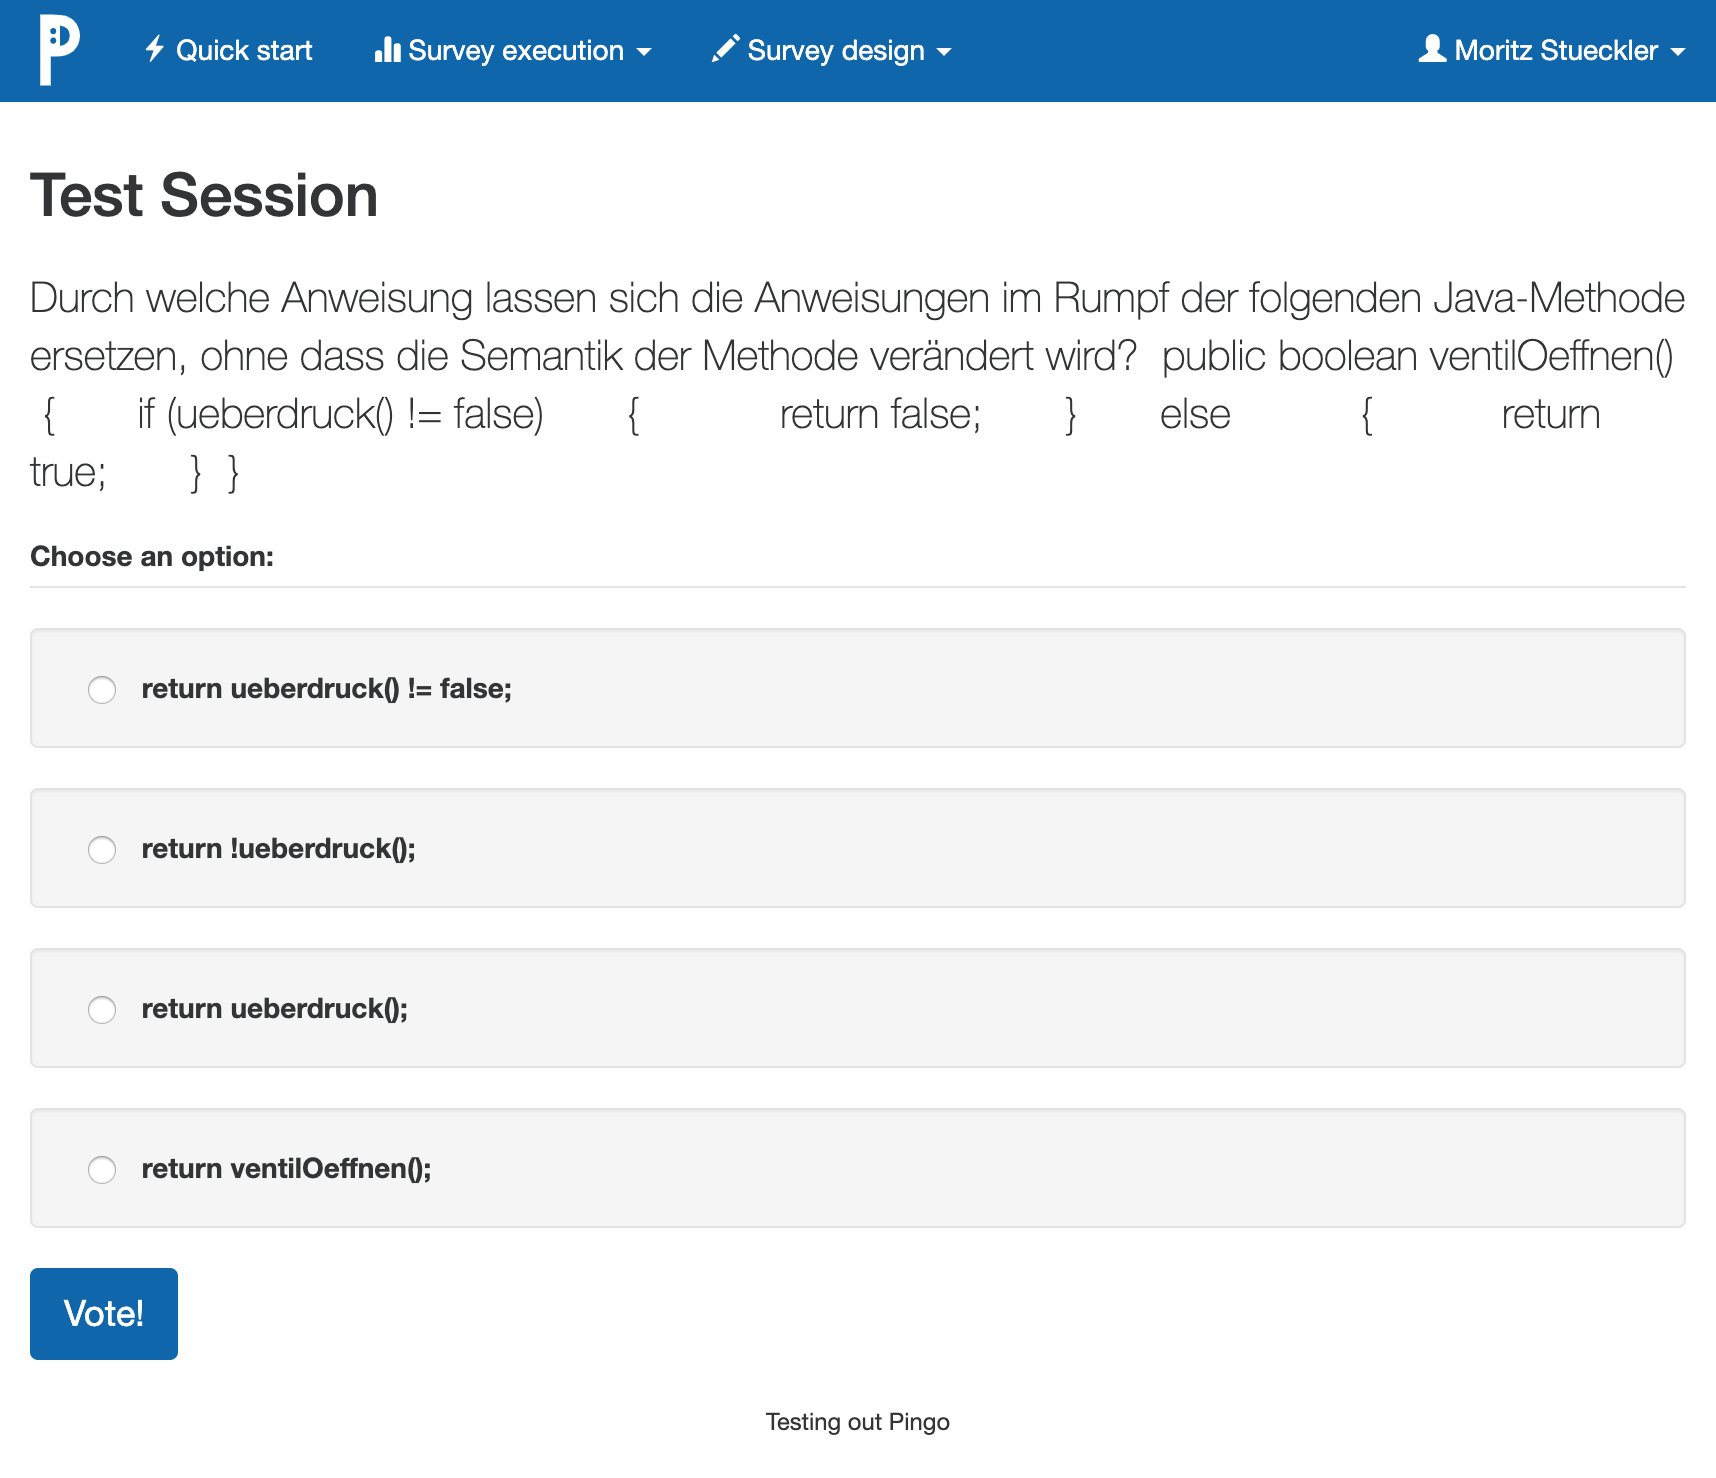
\includegraphics[width=12cm]{chapter/bewertung/bilder/pingo_problem1.png}
    \centering
    \caption{Pingo verfügt über keinerlei Text-Formatierungsoptionen und ist daher ungeeignet für die Darstellung von Quelltext.}
    \label{Abbildung 2.4}
\end{figure}
%
\chapter{Entwurf und Implementierung eines modernen CRS für die Programmierlehre}
\label{chap:entwurf}
Im Rahmen dieser Arbeit wird ein CRS entworfen und prototypisch implementiert, welches die besagten Kern-Anforderungen erfüllt. Die entstehende Software hört auf den Namen Weclare (ein Akronym für „\textbf{We}b \textbf{Cla}ssroom \textbf{Re}sponse (System)“. Der gesamte Quelltext zu dem Projekt findet sich in einem öffentlichen GitHub-Repository\cite{web:github_weclare} und eine öffentlich zugängliche Version der Software kann unter \texttt{www.weclare.de} aufgerufen werden. Insgesamt hat die entstandene Implementierung einen Umfang von rund 6000 Zeilen Code (vergleichbar mit dem Vorbild StuReSy).

Eine weitere Anforderung an das neue System: Zur Evaluierung soll Weclare auch mit bestehenden Datensätzen aus StuReSy funktionieren. Aus diesem Grund wird außerdem ein Kommandozeilen-Werkzeug entwickelt, welches Fragensätze vom XML-basierten StuReSy-Format in das JSON-basierte Weclare-Format konvertiert. Dieser Konverter wurde ebenfalls in JavaScript geschrieben und benötigt die Node.js-Laufzeitumgebung. Auch dieses Hilfsprogramm kann in einem öffentlichen GitHub-Repository\cite{web:github_converter} gefunden werden. 

\newpage
\section{Implementierung als Single Page Application mit dem React-Framework}
\label{chap:react_einfuehrung}
Um eine webbasierte Anwendung zu erstellen, die ohne einen zentralen Server auskommt, muss die Software komplett clientseitig in einem Browser ausgeführt werden, das heißt auch vollständig in JavaScript implementiert werden. Ein klassisches Backend, also eine Datenschicht (üblicherweise handelt es sich bei den meisten Web-Applikationen mindestens um eine Zwei-Schichten-Architektur) existiert nicht, beziehungsweise ist in die Präsentationsschicht integriert. Das bedingt die Kategorisierung einer solchen Anwendung als „Fat Client“.

Für diesen Zweck bietet es sich an, die Software als sogenannte „Single Page Application“ zu implementieren. Herkömmliche Webseiten, sogenannte Multi-Page-Applications werden während ihrer Lebenszeit mehrfach aktualisiert. Zum Beispiel jedes Mal, wenn der Server neues HTML liefert, das dargestellt werden soll. Eine Single Page Appliaction lädt nur eine einzige Webseite und das zugehörige JavaScript-Programm und verändert diese eine Seite dann im weiteren Verlauf dynamisch. Weitere Inhalte werden bei Bedarf asynchron (ohne Blockieren der Seite) nachgeladen, es wird jedoch keine neue Seite geladen. Damit wird auch eine hohe Autarkie gegenüber dem Webserver erreicht, da dieser nur mit wenigen Requests (im einfachsten Fall ein Request pro Nutzer) umgehen muss. Die Anforderungen an den Webserver auf dem die Anwendung bereitgestellt wird sind sehr gering, er muss lediglich statische Dateien (HTML, JavaScript, Bilder, Schriften, etc.) bereitstellen.

Als Framework für die Implementierung einer solchen Single Page Application wird das React-Framework\cite{web:react} ausgewählt. Das Open-Source-Projekt existiert seit 2013 und wird von Facebook finanziert. Es gehört zu den populärsten Frameworks zum Erstellen von Benutzeroberflächen und Web-Applikationen und ist dem Autor der Arbeit bereits vertraut.

Um einige Implementationsdetails nachzuvollziehen, erfolgt an dieser Stelle eine kleine Einführung in Grundkonzepte von React.

\subsection{Komponenten und State}
Die elementaren Bausteine einer React-Anwendung sind \texttt{Komponenten}. Die React-Dokumentation beschreibt die Aufgabe von Komponenten wie folgt\cite{web:react}:
\begin{quotation}
„Build encapsulated components that manage their own state, then compose them to make complex UIs.“
\end{quotation}

Ein Komponente ist eine autarke und wiederverwendbare Einheit und kapselt meistens sowohl Struktur, Aussehen als auch Logik. Komponenten werden häufig als Klasse implementiert (können aber in einfachen Fällen auch als Funktion implementiert werden) und erben von der Klasse \texttt{React.Component}. Valide Komponenten müssen über eine \texttt{render()}-Funktion verfügen, die HTML oder andere React-Komponenten zurückliefert. Eine sehr simple, statische Komponente könnte so aussehen:

\begin{minipage}{\linewidth}
\begin{lstlisting}[caption={Einfache React-Komponente ohne JSX-Syntax.}]
import React from "react";

class Greeting extends React.Component {
  render() {
    return React.createElement("div", null, "Hello there!");
  }
}
\end{lstlisting}
\end{minipage}

Da der Aufruf \texttt{React.createElement()} nicht so schön zu lesen ist, wie die Notation eines XML-Tags (\texttt{<div>...</div>}) wird im React-Umfeld häufig eine Syntax-Erweiterung namens JSX (JavaScript Syntax Extension) verwendet um React-Komponenten zu beschreiben. JSX wird mit einem Compiler während des Build-Prozesses in herkömmliches JavaScript umgewandelt. Äquivalent zum letzten Beispiel wäre daher die folgende Variante unter Einbeziehung von JSX-Syntax:

\begin{minipage}{\linewidth}
\begin{lstlisting}[caption={Einfache React-Komponente mit JSX-Syntax.}]
import React from 'react';

class Greeting extends React.Component {
    render() {
        return <div>Hello there!</div>;
    }
}
\end{lstlisting}
\end{minipage}

Um Komponenten dynamisch zu machen, können über sogenannte \texttt{Properties} Daten an Komponenten übergeben werden:

\begin{minipage}{\linewidth}
\begin{lstlisting}[caption={Komponenten erhalten Daten über ihre Properties.}]
import React from "react";

class Greeting extends React.Component {
  render() {
    return <div>Hello, {this.props.name}!</div>;
  }
}
\end{lstlisting}
\end{minipage}

Properties werden wie andere HTML-Attribute auch einfach hinter den Namen der Komponente innerhalb des zugehörigen Tags in die Instanziierung einer Komponente integriert:

\begin{minipage}{\linewidth}
\begin{lstlisting}[caption={Properties werden wie normale HTML-Attribute verwendet.}]
import React from "react";

class GreetAllFriends extends React.Component {
  render() {
    return (
      <div>
        <Greeting name="Michael" />
        <Greeting name="Karla" />
      </div>
    );
  }
}
\end{lstlisting}
\end{minipage}

\texttt{Properties} werden also verwendet um Daten in Komponenten hinein zu reichen. React kümmert sich automatisch um das Aktualisieren der aktuellen Ansicht, sobald sich eine Property ändert (dieses „reaktive“ Prinzip ist auch der Namensgeber für das Framework). Dabei verwendet React sehr schnelle und intelligente Algorithmen, um immer nur diejenigen Elemente einer Seite zu aktualisieren, die sich auch tatsächlich geändert haben.

Properties können nicht modifiziert werden – sie sind wie auch die meisten anderen Objekte innerhalb von React „immutable“. Wenn Daten innerhalb einer Komponente modifiziert werden sollen, gehören sie in das interne, modifizierbare \texttt{state}-Objekt dieser Komponente:

\begin{minipage}{\linewidth}
\begin{lstlisting}[caption={Jede Komponente kann über einen modifizierbaren state verfügen.}]
import React from "react";

class BusyOrNot extends React.Component {
  state = {
    busy: false
  };

  toggleBusy() {
    this.setState(prevState => ({
      busy: !prevState.busy
    }));
  }

  render() {
    return (
      <div>
        <div>This user is {busy ? "busy" : "not busy"}!</div>
        <button type="button" onClick={this.toggleBusy}>
          Change Busy State
        </button>
      </div>
    );
  }
}
\end{lstlisting}
\end{minipage}

Bedingt durch die statische Natur der Properties, forciert React einen unidirektionalen Datenfluss. Daten können nur von „oben nach unten“ (in Bezug auf die Baumstruktur im Document Object Model einer Seite) durch eine Anwendung fließen. Möchten zwei Komponenten an unterschiedlichen Stellen auf die gleichen Daten zugreifen, dann sollten diese in einer gemeinsamen Eltern-Komponente gehalten werden. \newline

\begin{minipage}{\linewidth}
\begin{lstlisting}[caption={„Lifting state up“: Mehrere Komponenten greifen auf die gleichen Daten zu.}]
import React from "react";

function Son(props) {
  return <p>I am the son of {props.parent}</p>
}

function Daughter(props) {
  return <p>I am the daughter of {props.parent}</p>
}

class Parent extends React.Component {
  state = {
    parentName: "Peter Parent"
  };

  render() {
    return (
      <div>
        <Son parent={this.state.parentName} />
        <Daughter parent={this.state.parentName} />
      </div>
    );
  }
}
\end{lstlisting}
\end{minipage}

Da dieses Muster bei großen Anwendungen aber schnell zu sehr aufwendigem „Durchstecken“ von Properties (Prop Drilling) durch mehrere Komponenten-Ebenen führt, gibt es eine populäre Erweiterung für React zur Verwaltung eines globalen States in der gesamten Anwendung: das Flux-Muster.


\subsection{State Management mit Redux}
Das Flux-Entwurfsmuster ist ebenfalls eine Entwicklung von Facebook. Prinzipiell handelt es sich um ein abstraktes Entwurfsmuster, das in vielen Sprachen angewendet werden kann. Etabliert hat es sich jedoch gerade in Kombination mit React-Anwendungen. Die bekannteste Implementation, die auch in dieser Arbeit verwendet wird, hört auf den Namen Redux \cite{web:redux}.

Im Flux-Muster geht es darum, eine zentrale Zustandsverwaltung für eine Anwendung einzurichten, eine sogenannte „Single Source of Truth“. Dieser zentrale Ort wird als „Store“ bezeichnet. Ein Store beinhaltet typischerweise solche Daten, die für die gesamte Anwendung relevant sind. Parallel dazu kann es aber weiterhin Komponenten geben, die einen eigenen, lokalen State verwalten, wenn dieser nicht für die gesamte Anwendung relevant ist (zum Beispiel der Status von einzelnen UI-Elementen).

\begin{figure}[H]
    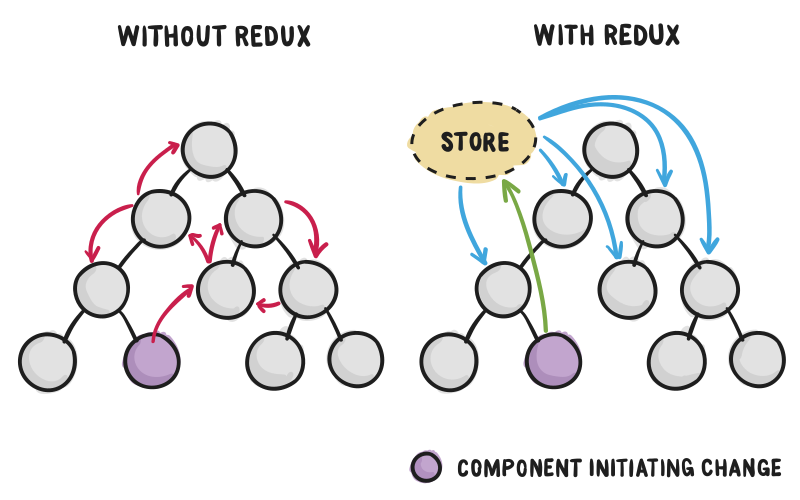
\includegraphics[width=12cm]{chapter/entwurf/BA_redux.png}
    \centering
    \caption{Der Redux-Store verwaltet den globalen Zustand einer React-Anwendung und ist die „Single Source of Truth“. Quelle: https://css-tricks.com/learning-react-redux/ (aufgerufen am 24.4.19)}
    \label{Abbildung 4.1.3}
\end{figure}


Einzelne React-Komponenten können mit einem Store durch einen Publish/Subscribe-Mechanismus verbunden werden. Die gewünschten Daten aus dem Store stehen der Komponente dann als Properties zur Verfügung. Ändern sich die Daten im Store, dann wird die verbundene Komponente sofort benachrichtigt und bei einer Änderung der Properties auch neu gerendert (reaktives Prinzip). Um eine möglichst lose Kopplung zwischen den Komponenten zu realisieren, wird empfohlen die Verbindung zu einem Store in einer (nicht sichtbaren) Container-Komponente zu realisieren. In diesem Beispiel wird die eigentliche, sichtbare \texttt{Header}-Komponente mit einem unsichtbaren Container versehen, der die notwendigen Daten aus dem Store innerhalb der Komponente unter der \texttt{status}-Property verfügbar macht.

\begin{minipage}{\linewidth}
\begin{lstlisting}[caption={Über den connect-Aufruf beim Exportieren der Komponente wird sie mit dem Store verbunden.}]
import { connect } from "react-redux";
import Header from "./Header";

const mapStateToProps = state => ({
  status: state.connection.status
});

export default connect(mapStateToProps)(Header);
\end{lstlisting}
\end{minipage}

Ähnlich wie die Properties in React, sind auch die Daten in einem Store unveränderlich. Änderungen in einem Store müssen mithilfe von \texttt{Actions} realisiert werden. Bei einer Action handelt es sich lediglich um ein Objekt, welches die Art der Änderung in einem Store beschreibt. Um das wiederholte Schreiben aufwändiger Objekt-Literale zu erleichtern werden die Actions üblicherweise von einer \texttt{ActionCreator}-Funktion erzeugt:

\begin{minipage}{\linewidth}
\begin{lstlisting}[caption={Ein Action-Objekt ist lediglich die Beschreibung einer Änderungsoperation und wird in einem ActionCreator erzeugt.}]
export function addQuestion(newQuestion) {
  return {
    type: "ADD_QUESTION",
    payload: {
      newQuestion
    }
  };
}
\end{lstlisting}
\end{minipage}

Die Implementierung einer Änderungsoperation erfolgt in dem zugehörigen \texttt{reducer}. Die Operationen in einem reducer sind stets pure Funktionen, das heißt sie liefern immer das gleiche Ergebnis bei gleichen Eingabe-Parametern und sie haben keine Seiteneffekte. Die Parameter des reducers sind immer der aktuelle State und die eingehende Action. Ein einfacher Reducer zum Hinzufügen einer Frage zu einem Fragekatalog könnte so aussehen:

\begin{minipage}{\linewidth}
\begin{lstlisting}[caption={In einem Reducer werden die Änderungsoperationen eines Stores als pure Funktion implementiert.}]
const questionEditor = (state = [], action) => {
  switch (action.type) {
    case "ADD_QUESTION": {
      return [... state, createNewQuestion()];
    }
  }
};
\end{lstlisting}
\end{minipage}

\subsection{Konkrete Umsetzung am Beispiel des Fragen-Editors}
Um das neue CRS zu implementieren, muss zuerst eine sinnvolle Aufteilung in Komponenten erfolgen. Exemplarisch soll an dieser Stelle einer der Hauptbestandteile der Anwendung besprochen werden: der Fragen-Editor.

Das zweiteilige Design, bestehend aus einer Fragenliste in der Seitenspalte und einem Fragen-Inhaltsbereich, das sowohl bei StuReSy als auch bei Pingo zum Einsatz kommt, soll beibehalten werden.

Eine mögliche Komponenten-Hierarchie für den Fragen-Editor wird in \ref{Abbildung 4.1} veranschaulicht. Die äußerste Komponente, der \texttt{QuestionEditorContainer} ist nicht sichtbar, es handelt sich dabei um eine Container-Komponente, welche die notwendigen Daten aus dem Store holt und dann an seine Kinder-Komponenten mittels Properties weitergibt.

\begin{figure}[H]
    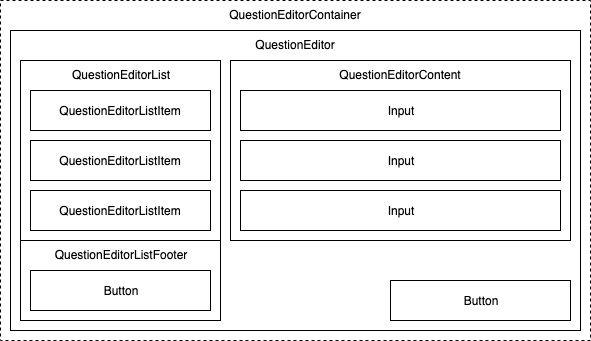
\includegraphics[width=12cm]{chapter/entwurf/Component_Hierarchy.png}
    \centering
    \caption{Mögliche Komponenten-Hierarchie für den Fragen-Editor.}
    \label{Abbildung 4.1}
\end{figure}

Die tatsächliche Implementierung entspricht nahezu vollständig diesem Bild (einzig die Komponente \texttt{QuestionEditorListItem} findet sich nicht im fertigen Ergebnis.

\begin{figure}[H]
    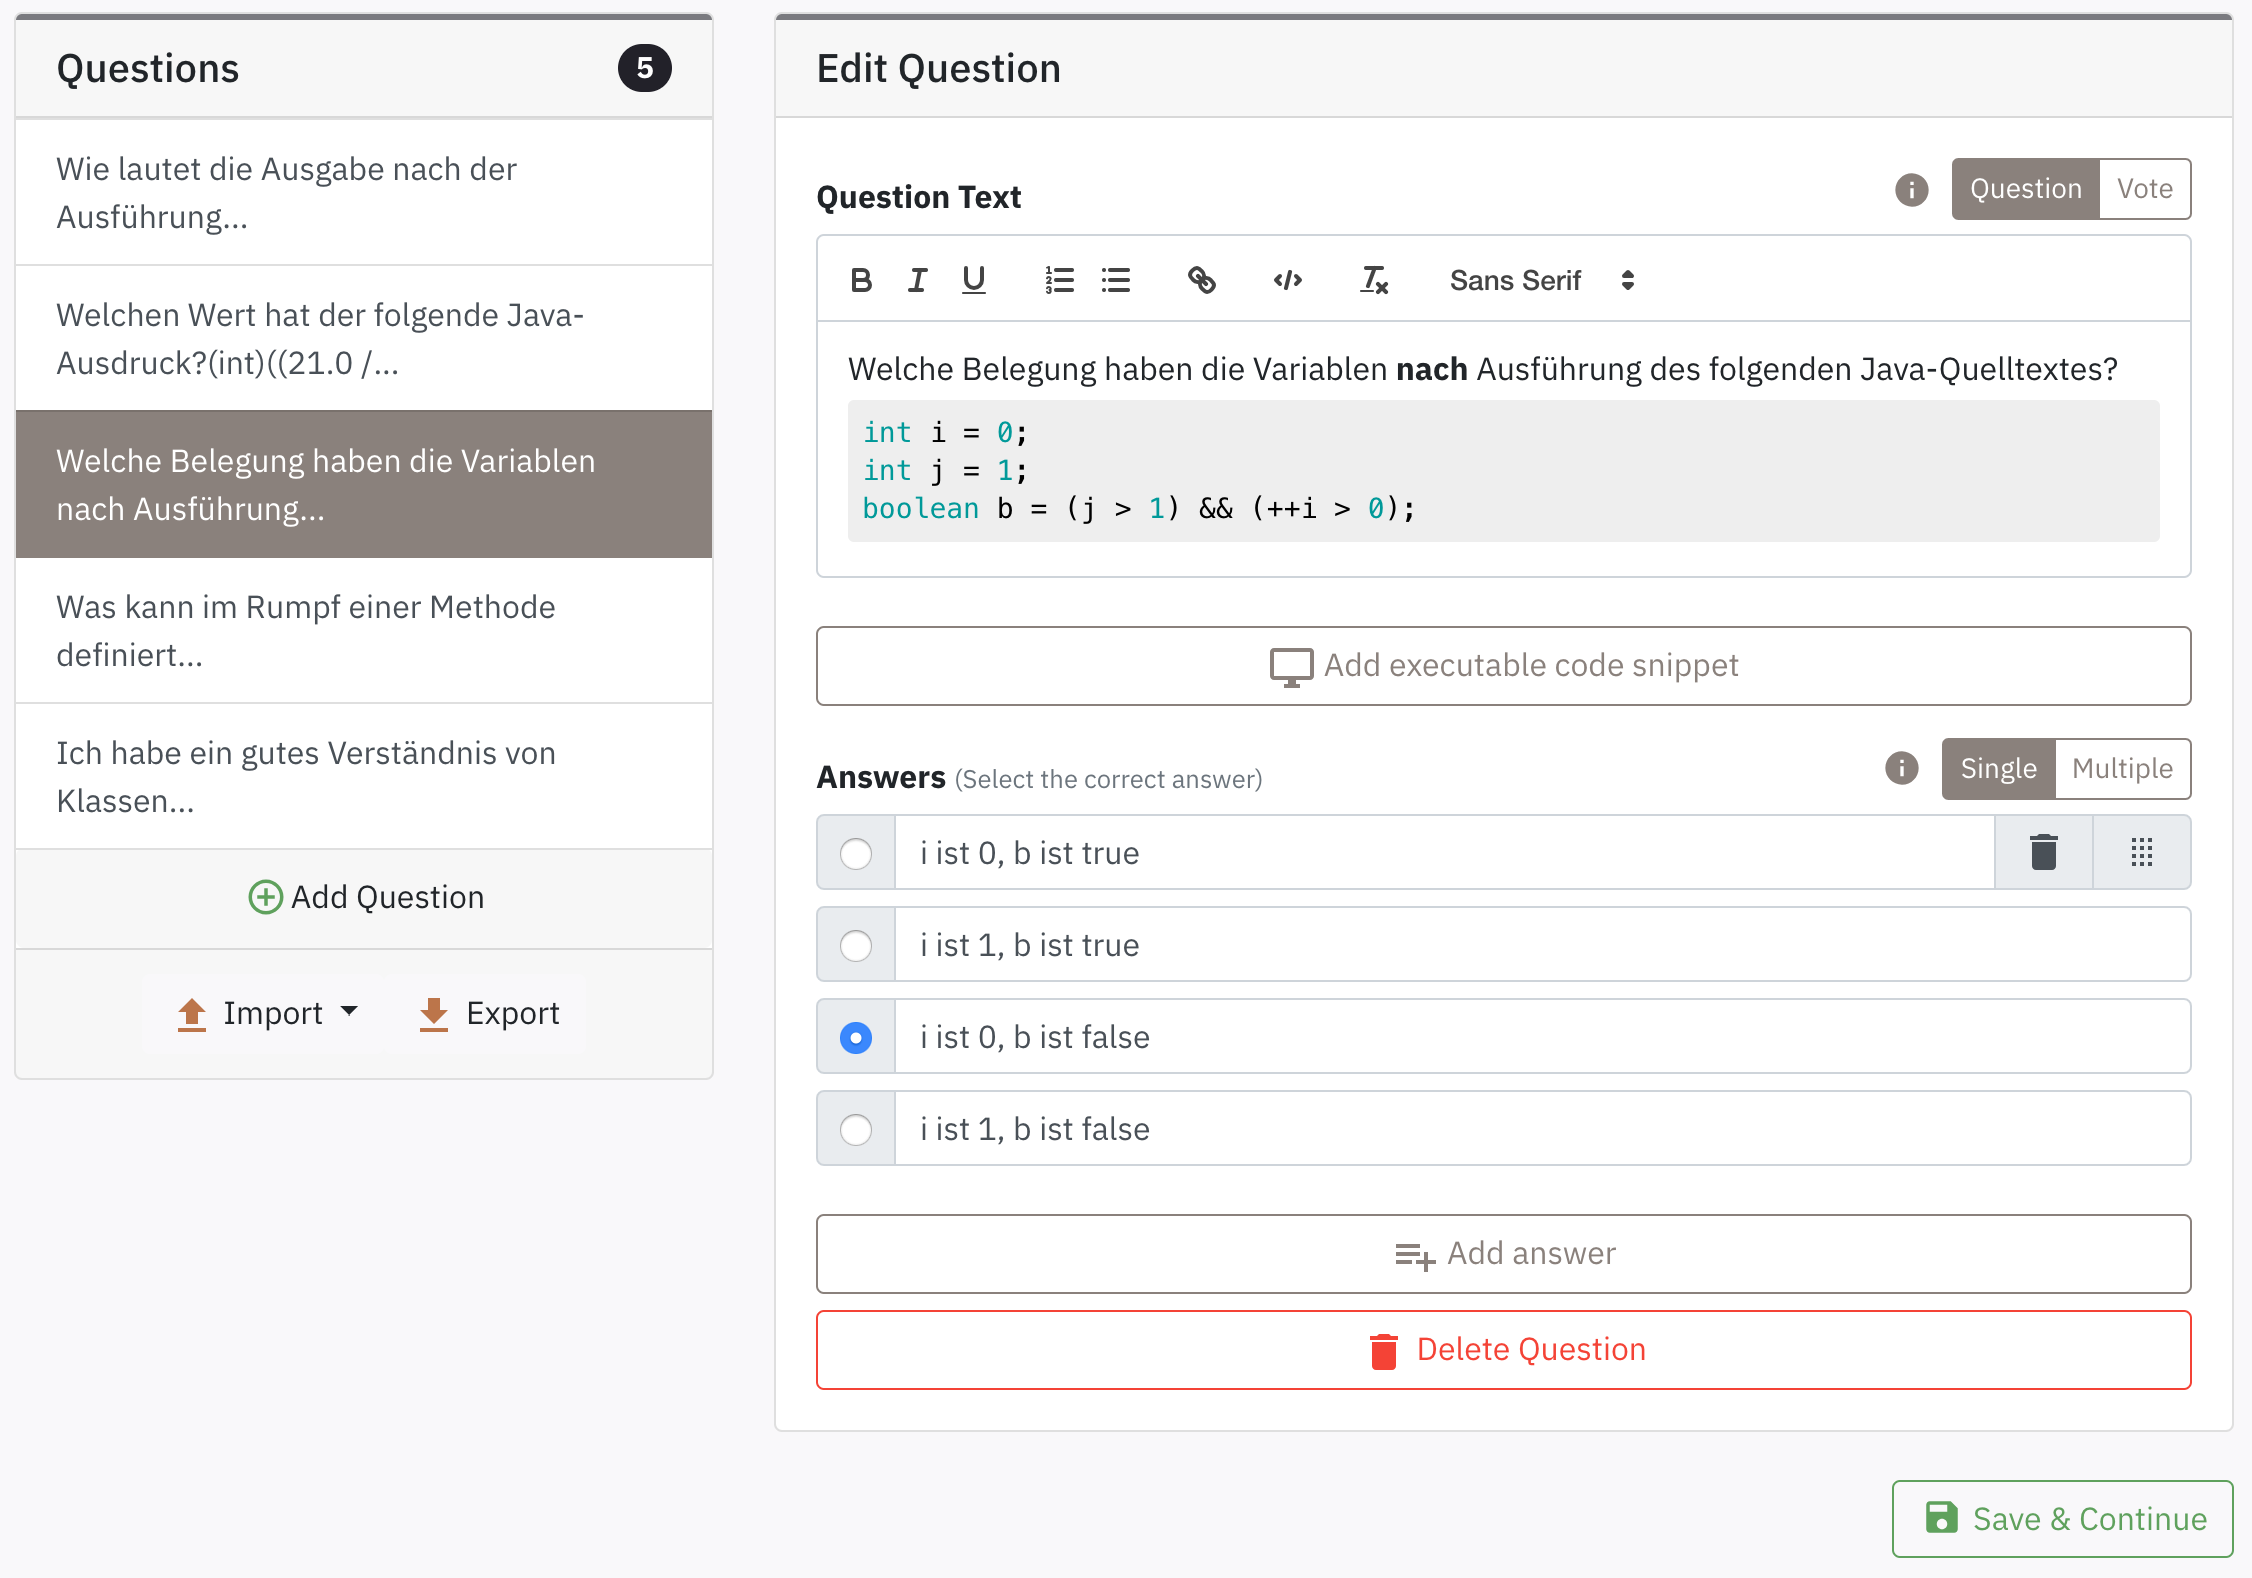
\includegraphics[width=16cm]{chapter/entwurf/weclare_editor.png}
    \centering
    \caption{Fertige Implementierung des Fragen-Editors im React-Framework.}
    \label{Abbildung 4.2}
\end{figure}

Alle Daten des Fragen-Editors werden in einem einzigen Redux-Store gehalten. Alle möglichen Änderungen finden sich in einem zugehörigen Reducer wieder, der auszugsweise wie folgt aussieht:


\begin{minipage}{\linewidth}
\begin{lstlisting}[caption={Auszug aus dem Reducer für den Fragen-Editor.}]
export const questionEditor = (state = [], action) => {
  switch (action.type) {
    case ADD_QUESTION: {...}
    case EDIT_QUESTION_TEXT: {...}
    case EDIT_QUESTION_CODE: {...}
    case EDIT_QUESTION_MODE: {...}
    case EDIT_QUESTION_TYPE: {...}
    case DELETE_QUESTION: {...}
    case DELETE_ANSWER: {...}
    case ADD_ANSWER: {...}
    case EDIT_ANSWER_TEXT: {...}
    case SET_CORRECT_SINGLE_ANSWER: {...}
    case SET_CORRECT_MULTI_ANSWER: {...}
    case LOAD_QUESTIONS: {...}
    case SORT_QUESTION: {...}
    case SORT_ANSWER: {...}
    default: {
      return state;
    }
  }
};
\end{lstlisting}
\end{minipage}


\newpage
\section{P2P-WebRTC-Verbindungen mit PeerJS}
\label{chap:p2p}
Um Unabhängigkeit von einem dedizierten, zentralen Anwendungsserver zu erlangen, der einerseits Wartungsaufwand bedeutet, und außerdem einen „Single Point of Failure“ darstellt, werden Verbindungen direkt zwischen den Teilnehmern aufgebaut. Jeder Weclare-Nutzer kann zum Start einer Sitzung, also zur Laufzeit, entscheiden, welche Rolle er in der aktuellen Sitzung einnehmen will (Server oder Client). Der Rechner des Dozenten agiert typischerweise als Server, die Rechner der Studenten sind Clients und somit ergibt sich eine klassische, zentralisierte Architektur des verteilten Systems in Form einer Stern-Topologie. Unabhängig von der Wahl wird jedoch stets der gleiche Code vom Server geladen. Das Programm ist in dieser Hinsicht also omnipotent.

\begin{figure}[H]
    \centering
    \setlength{\fboxsep}{0pt}
    \setlength{\fboxrule}{0.5pt}
    \fbox{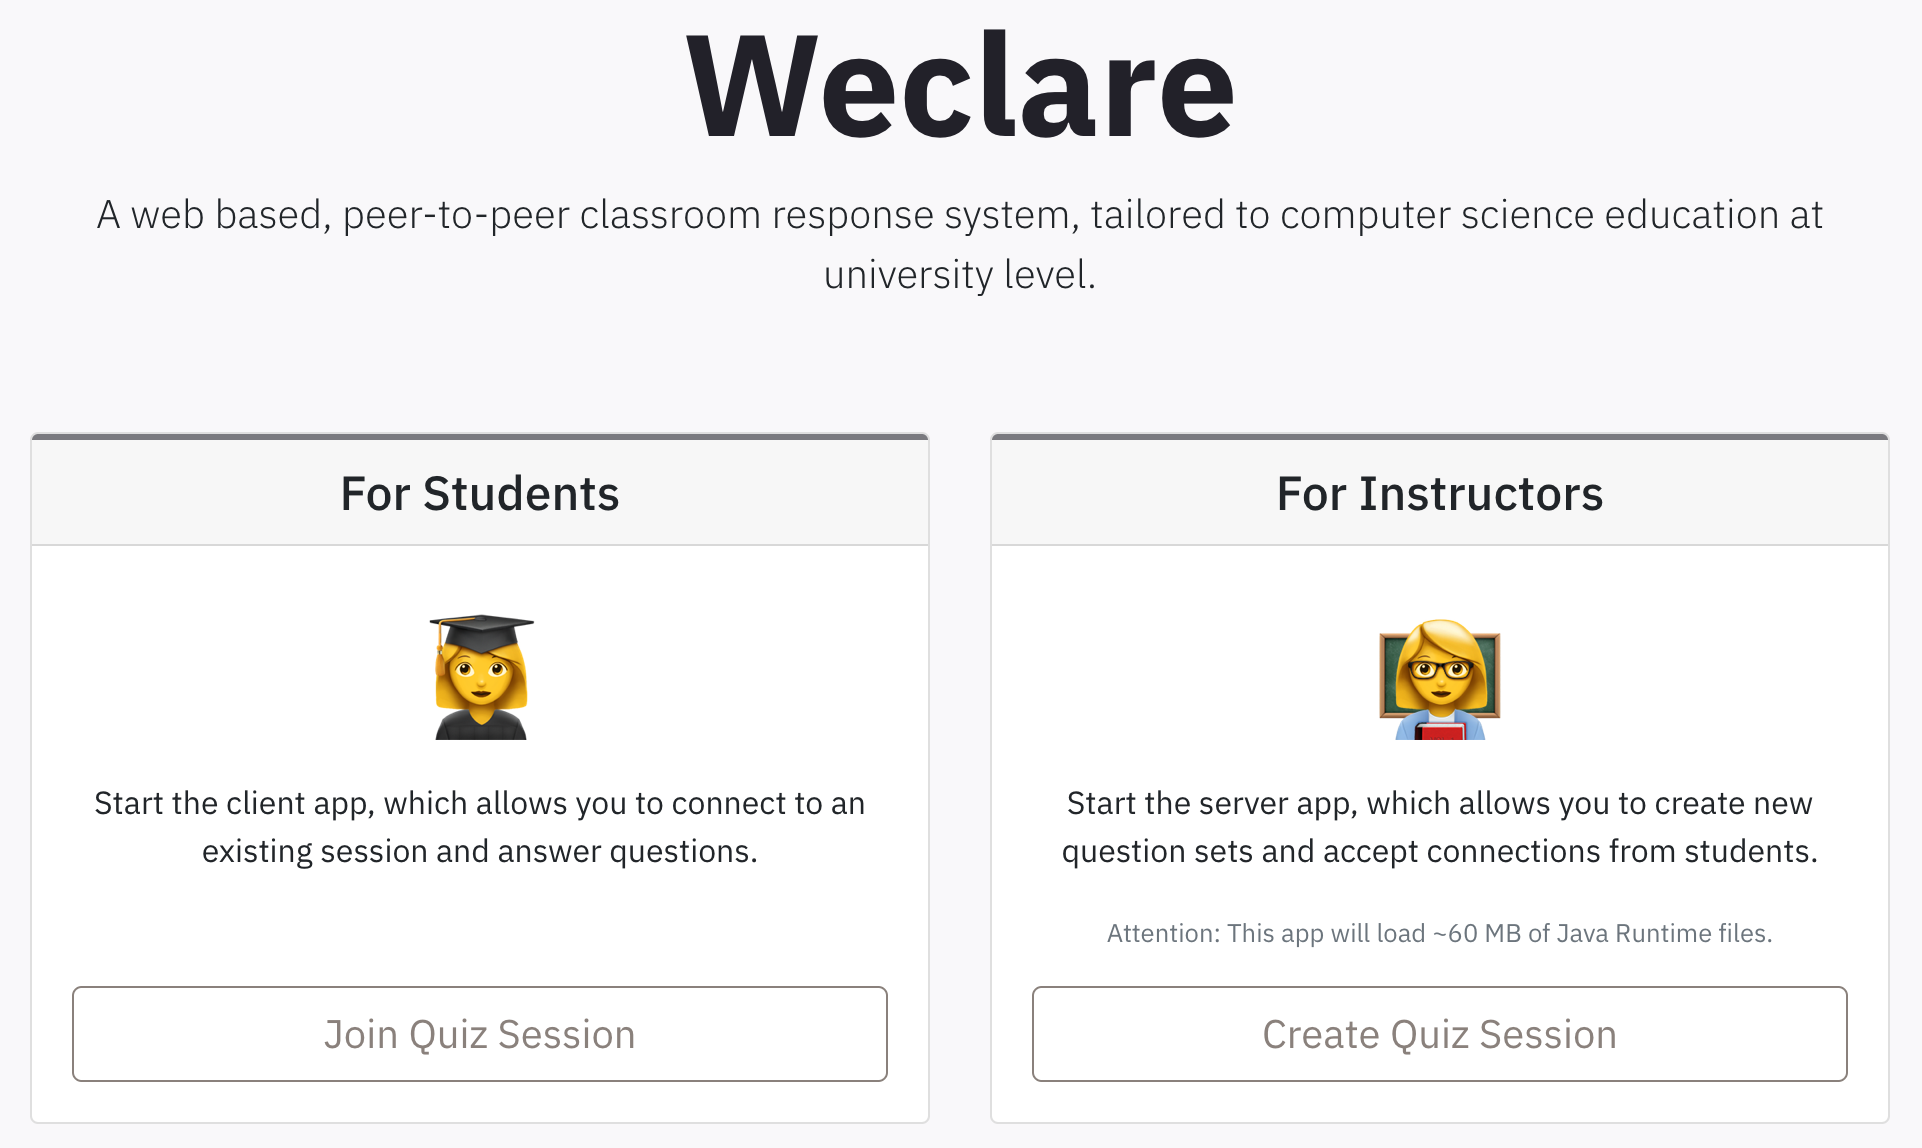
\includegraphics[width=\textwidth-1pt]{chapter/entwurf/bilder/weclare_start.png}}
    \caption[Start einer neuen Weclare-Sitzung]{Am Start einer Sitzung kann der Nutzer entscheiden, ob er als Client oder als Server teilnehmen möchte. Unabhängig von der Wahl wird das gleiche Programm geladen.}
    \label{abb:weclare_start}
\end{figure}

Mit diesem Verhalten erfüllt die Software die Definition einer Peer-to-Peer Architektur, zum Beispiel gemäß Tanenbaum\cite[S. 62]{book:tanenbaum}:

\begin{quotation}
„Aus einem übergeordneten Blickwinkel heraus sind die Prozesse, die ein Peer-to-Peer-System bilden, alle gleich. Die Funktionen, die ausgeführt werden müssen, werden also von jedem Prozess des verteilten Systems dargestellt. Folglich ist die meiste Interaktion zwischen Prozessen symmetrisch: Jeder Prozess agiert gleichzeitig als Client und als Server [...].“
\end{quotation}

Jedoch trifft dies nur auf den Zeitraum vor dem Start einer Sitzung zu. Sobald eine Sitzung begonnen hat, handelt es sich um eine klassische Client-Server-Struktur. Die Bezeichnung als Peer-to-Peer-Architektur entspricht daher nicht der gängigen Vorstellung eines vollvermaschten Peer-to-Peer-Netzwerks, bei dem jeder Teilnehmer mit jedem anderen Teilnehmer verbunden ist.

Die Tatsache, dass jeder Teilnehmer entscheiden kann, ob er als Server oder Client teilnehmen will, bedeutet auch, dass Aspekte wie Network Address Translation (NAT) und Firewalls beim Austausch der IP-Adressen (Signaling) berücksichtigt werden müssen.

Der Zugriff auf die Schnittstellen des Betriebssystems (wie etwa das Netzwerk) durch Browser-Skripte ist aus Sicherheitsgründen stark eingeschränkt. Viele bestehende webbasierte CRS (zum Beispiel Pingo, vgl. \cite{web:pingo_github}) verwenden das WebSocket-Protokoll zur Kommunikation zwischen Client und Server. Der WebSocket-Standard beschreibt jedoch nur Möglichkeiten zum Verbinden mit einem bestehenden Server aus dem Browser heraus, nicht zum Kreieren einer Verbindung (vgl. \cite{std:websockets}). Eine Peer-to-Peer-Architektur mit WebSockets ist deswegen nicht realisierbar.

Die einzige Möglichkeit, eine omnidirektionale Verbindung zwischen zwei Browsern zu realisieren, ist der relativ neue und offene WebRTC-Standard (Web Real-Time Communication)\footnote{Offizielle Webseite: \url{https://webrtc.org/}}. WebRTC wird hauptsächlich für Multimedia-Echtzeit-Anwendungen eingesetzt und seit 2017 von allen großen Browsern (Google Chrome, Mozilla Firefox, Opera, Apple Safari und Microsoft Edge) unterstützt. Viele Video- und Audiotelefonie-Lösungen (zum Beispiel Skype oder Discord) basieren inzwischen auf dem WebRTC-Protokoll. Neben Audio- und Videoinhalten können aber auch beliebige andere Daten über sogenannte \texttt{RTCDataChannel} übertragen werden. WebRTC beinhaltet keine Anweisungen für den Austausch der IP-Adressen zwischen beteiligten Parteien. Dieser Teil, das sogenannte Signaling, ist nicht Teil des Standards und muss selbst implementiert werden (vgl. \cite{web:webrtc_signaling}).

Der Aufwand dafür ist groß, weil viele verschiedene Netzwerk-Situationen berücksichtigt werden müssen. Deswegen wird beim Weclare-Prototypen eine OpenSource-Bibliothek namens PeerJS\footnote{Offizielle Webseite: \url{https://peerjs.com/}} verwendet, die WebRTC in eine sehr einfache API kapselt und ein Signaling-Verfahren beisteuert.

Die (in Kapitel \ref{chap:anforderung_p2p}) formulierte Anforderung, keinen dedizierten Server zu benötigen, kann aufgrund des notwendigen Signalings also nicht vollständig erfüllt werden und muss präzisiert werden: Ein Server wird lediglich zum Austausch der IP-Adressen der Teilnehmer benötigt. Nach dem Austausch ist kein Server mehr notwendig. Anwendungsdaten werden nie über einen zentralen Server, sondern immer nur zwischen den einzelnen Teilnehmern verschickt. Der notwendige Signaling-Server muss nicht vom Weclare-Anwender betrieben werden – ein öffentlicher Server kann verwendet werden. In der Standard-Einstellung verwendet PeerJS einen kostenlosen und öffentlichen Signaling-Server, der von den PeerJS-Autoren betrieben wird.

Die PeerJS-Library ermöglicht den Aufbau einer Datenverbindung zwischen zwei Browsern mit sehr simplen Aufrufen: Zunächst müssen Client und Server ein Peer-Objekt erzeugen. Als Parameter kann an dieser Stelle eine (auf dem Signaling-Server noch nicht verwendete) alphanumerische ID übergeben werden, unter welcher der zugehörige Peer beim Signaling-Server bekannt gemacht wird. Optional kann hier außerdem ein eigener Signaling-Server angegeben werden. 

Anschließend können an dem neuen Peer-Objekt diverse Callback-Methoden registriert werden, die den weiteren Gebrauch regeln. So kann zum Beispiel der Server seine neu erstellte ID kundtun und auf eingehende Verbindungen und Daten reagieren:

\begin{minipage}{\linewidth}
\begin{lstlisting}[caption={Verbindungsaufbau mit der PeerJS-Bibliothek auf der Server-Seite. (aus: src/server/actions/server.js)}]
import Peer from "peerjs";

const peer = new Peer("server-id");

peer.on("open", id => {
  console.log(`Successfully created peer: ${id}`);
});

peer.on("connection", conn => {
  console.log(`New client connected: ${conn.peer}`);
  conn.on("data", data => {
    switch (data.type) {
      case "answer":
        // Do something
        break;
      default:
      // Noop
    }
  });
});
\end{lstlisting}
\end{minipage}

Auf der Gegenseite, beim Client kann die Verbindung einfach über die \texttt{connect()}-Methode aufgebaut werden, die als Parameter die ID des gewünschten Peers erhält. Anschließend kann über das zurückgelieferte \texttt{Connection}-Objekt eine Nachricht verschickt werden. (vgl. \cite{web:peerj_docs})

\begin{minipage}{\linewidth}
\begin{lstlisting}[caption={Verbindungsaufbau mit der PeerJS-Bibliothek auf der Client-Seite. (aus: src/client/actions/client.js)}]
import Peer from "peerjs";

const peer = new Peer();
const connection = peer.connect("server-id");
connection.send("Hello world!");
\end{lstlisting}
\end{minipage}

Um dem Flux-Muster (siehe Kapitel \ref{chap:redux_state_management}) treu zu bleiben, wird die gesamte Netzwerk-Kommunikation innerhalb von ActionCreator-Funktionen implementiert. Da Netzwerk-Aufrufe keine puren Funktionen sind und asynchron erfolgen müssen, können sie nicht in einen Reducer integriert werden. Um solche asynchronen Actions zu realisieren, wird Redux um eine sehr simple Middleware namens \texttt{redux-thunk}\footnote{Offizielle Webseite: \url{https://github.com/reduxjs/redux-thunk}} erweitert. Diese Middleware erlaubt es, asynchrone Aufrufe in ActionCreator-Methoden unterzubringen (vgl. \cite{web:redux_async_actions}). Da viele dieser Netzwerkaufrufe eigentlich keine Änderungen im Store bewirken, wird der ActionCreator seinem Namen nicht mehr treu, denn am Ende wird, entgegen seinem Zweck, keine Action mehr zurückgegeben.

\begin{minipage}{\linewidth}
\begin{lstlisting}[caption={ActionCreator zum Versenden von Antworten vom Client zum Server. (aus: src/client/actions/client.js)}]
export function sendAnswers(answerIdxArray) {
  return (dispatch, getState) => {
    const {
      client: { connection = null, currentQuestion = null }
    } = getState();

    if (
      connection &&
      currentQuestion &&
      typeof answerIdxArray !== "undefined"
    ) {
      const msg = {
        type: "answer",
        payload: {
          questionIdx: currentQuestion.questionIdx,
          answerIdxArray,
          userId: connection.provider.id
        }
      };
      connection.send(msg);
    }
  };
}
\end{lstlisting}
\end{minipage}


\newpage
\section{Text- und Code-Formatierung mit Quill und CodeMirror}
\label{chap:formatierung}
Quelltexte können in zwei verschiedenen Kontexten in Fragestellungen auftauchen: Einerseits gibt es unvollständige, kurze Quelltext-Fragmente, die in einen Fließtext eingebunden werden sollen, wie in diesem Beispiel:

\begin{quote}
„Wie viele String-Parameter hat die folgende Java-Methode?\newline
public String m(int i, int s, boolean b) \{ ... \}“
\end{quote}

Dabei handelt es sich nicht um ein syntaktisch nicht vollständiges und nicht-ausführbares Java-Fragment. Um die Lesbarkeit dieses Fragments zu erhöhen, sollte es dennoch optisch deutlich vom Fließtext unterscheidbar sein. Es bietet sich an, den Code in einer Monospace-Schriftart zu formatieren und (wenn möglich) eine syntaktische Einfärbung (Syntax Highlighting) anzuwenden.

Da die Entwicklung einer eigenen Editor-Komponente komplex ist, und es in diesem Bereich bereits eine große Auswahl an Bibliotheken gibt, wird auf eine bestehende Implementierung zurückgegriffen. Dabei müssen folgende Anforderungen von einer solchen Bibliothek erfüllt werden:

\begin{itemize}
    \item \textbf{Integration in React:}  Muss sich leicht in das deklarative React-Framework einbinden lassen.
    \item \textbf{WYSIWYG (What You See Is What You Get):} Der Editor muss stets eine Vorschau aller Formatierungen darstellen, und es soll nicht zwischen einem Markup- und einem Vorschau-Modus gewechselt werden müssen. Formatierungen sollen über Buttons eingefügt werden können.
    \item \textbf{Text-Formatierungen:} Der Editor muss über simple Text-Formatierungen verfügen (zum Beispiel Fettschrift und Kursivierung).
    \item \textbf{Monospace-Schriftart:} Eine Möglichkeit zum Verwenden einer Monospace-Schriftart muss vorhanden sein.
    \item \textbf{Syntax-Highlighting:} Syntaktische, farbliche Hervorhebungen von Code-Fragmenten müssen unterstützt werden (üblicherweise durch ein Plugin/Erweiterung mit einer zusätzlichen Bibliothek wie Highlight.js).
\end{itemize}

Nach dem Erwägen und Ausprobieren diverser Bibliotheken (zum Beispiel Draft.js, Slate, Prosemirror, Quill) fiel die Wahl letztendlich auf den Quill-Editor\footnote{Offizielle Webseite: \url{https://quilljs.com/}}, der alle genannten Anforderungen erfüllt. Quill ist nicht primär für den Einsatz mit React vorgesehen, deswegen wird der Editor in Form der Wrapper-Bibliothek \texttt{react-quill}-Bibliothek\footnote{Offizielle Webseite: \url{https://github.com/zenoamaro/react-quill}} verwendet, die Quill in React-Komponenten bündelt.

\begin{figure}[H]
    \centering
    \setlength{\fboxsep}{0pt}
    \setlength{\fboxrule}{0.5pt}
    \fbox{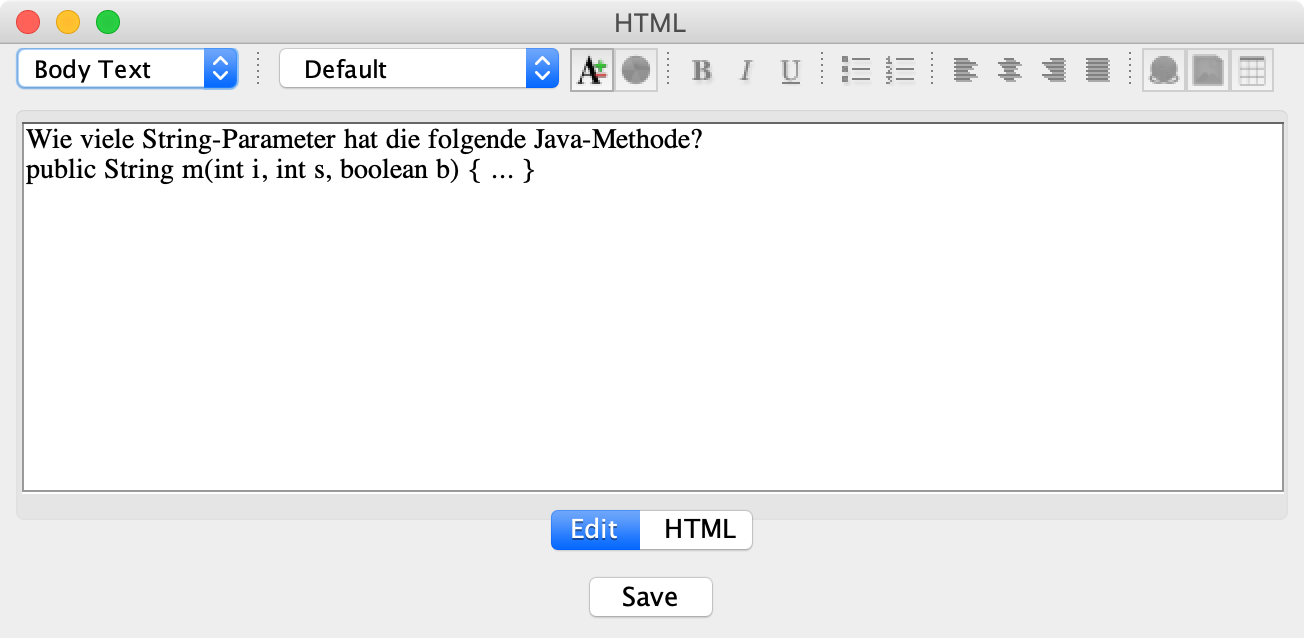
\includegraphics[width=\textwidth-1pt]{chapter/entwurf/bilder/sturesy_editor.png}}
    \caption[StuReSy-Fragen-Editor]{Bearbeiten einer Fragestellung im StuReSy-Fragen-Editor.}
    \label{abb:sturesy_editor}
\end{figure}

\begin{figure}[H]
    \centering
    \setlength{\fboxsep}{0pt}
    \setlength{\fboxrule}{0.5pt}
    \fbox{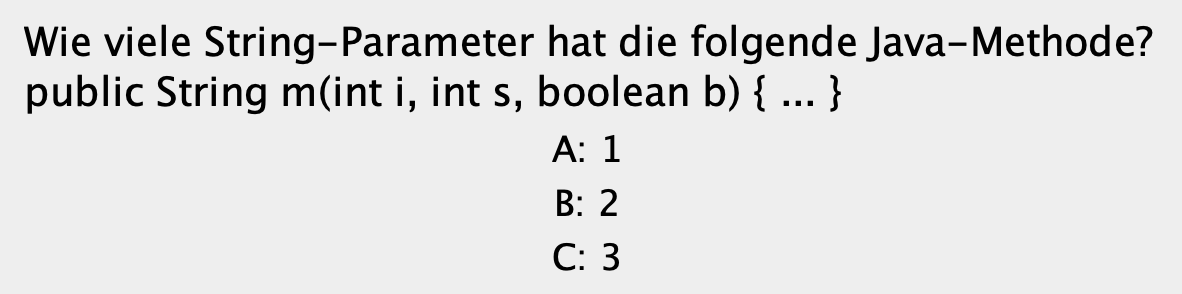
\includegraphics[width=\textwidth-1pt]{chapter/entwurf/bilder/sturesy_fragment.png}}
    \caption[Darstellung eines Code-Fragments in StuReSy]{Darstellung eines Code-Fragments in StuReSy (ohne manuell vorgenommene Formatierungen)}
    \label{abb:sturesy_code_fragment}
\end{figure}


\begin{figure}[H]
    \centering
    \setlength{\fboxsep}{0pt}
    \setlength{\fboxrule}{0.5pt}
    \fbox{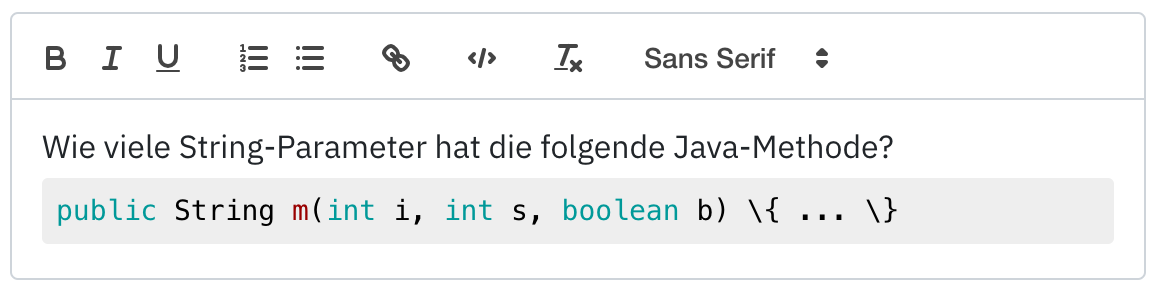
\includegraphics[width=\textwidth-1pt]{chapter/entwurf/bilder/weclare_quill.png}}
    \caption[Quill-Editor von Weclare]{Bearbeiten einer Fragestellung im Quill-Editor von Weclare.}
    \label{abb:weclare_quill}
\end{figure}

\begin{figure}[H]
    \centering
    \setlength{\fboxsep}{0pt}
    \setlength{\fboxrule}{0.5pt}
    \fbox{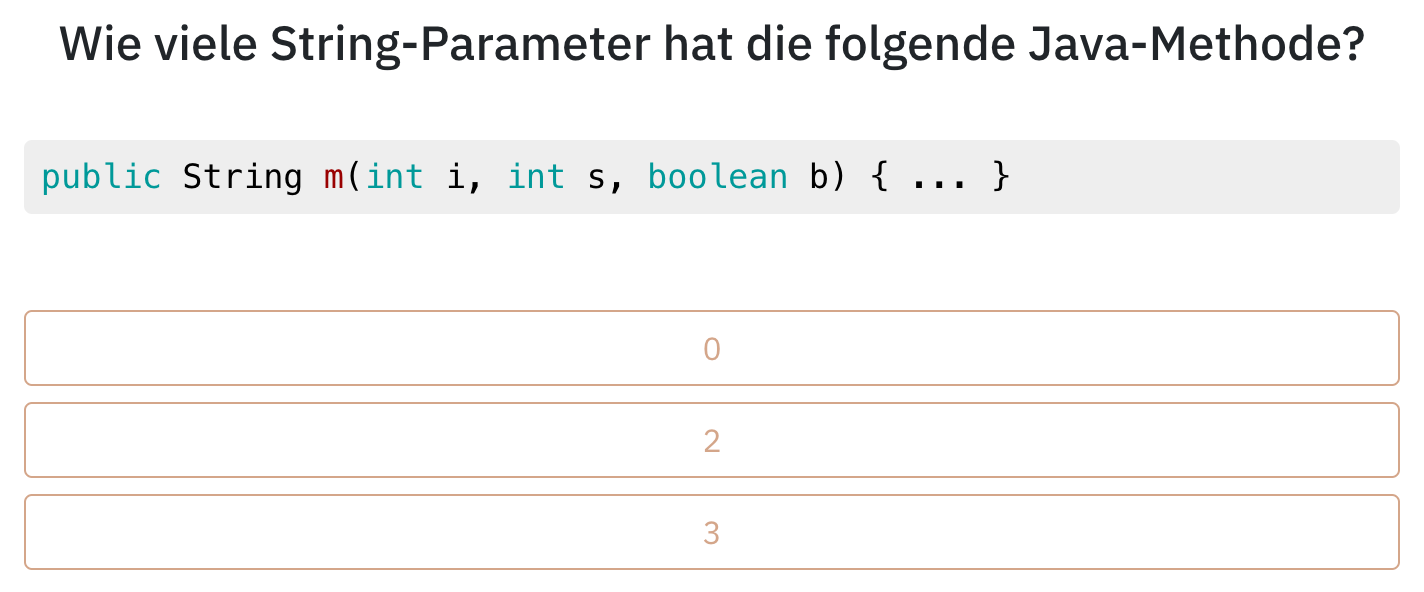
\includegraphics[width=\textwidth-1pt]{chapter/entwurf/bilder/weclare_fragment.png}}%
    \caption[Darstellung eines Code-Fragments in Weclare]{Darstellung eines Code-Fragments in Weclare (Quelltext als Code-Block ausgezeichnet)}
    \label{abb:weclare_code_fragment}
\end{figure}

Der zweite Kontext von Quelltexten in Fragestellungen ist das Einfügen von vollständigem, ausführbarem Code, in Form ganzer Java-Klassen. Solcher Code kann in Weclare direkt im Browser ausgeführt werden. So ein interaktives Code-Beispiel kann allerdings nur einmal pro Frage vorhanden sein und ist auch nicht Teil des Fließtexts. Eine entsprechende Editor-Komponente zum Einfügen solchen Codes sollte also auch funktional darauf zugeschnitten sein: Text-Formatierungen sind nicht mehr notwendig, stattdessen rücken Funktionen wie die korrekte Einrückung von Code-Zeilen und Zeilen-Nummerierungen in den Vordergrund.

Der Quill-Editor kann leider nicht in einem „Code only“-Modus betrieben werden, so dass eine zweite, unabhängige Editor-Komponente für interaktive Code-Abschnitte integriert wird. Mit CodeMirror\footnote{Offizielle Webseite: \url{https://codemirror.net/}} existiert eine sehr beliebte Bibliothek für diesen Zweck, die allerdings auch nicht explizit für den Einsatz im React-Framework bestimmt ist, so dass auch sie in Form einer Wrapper-Bibliothek namens \texttt{react-codemirror2}\footnote{Offizielle Webseite: \url{https://github.com/scniro/react-codemirror2}} zum Einsatz kommt.



\begin{figure}[H]
    \centering
    \setlength{\fboxsep}{0pt}
    \setlength{\fboxrule}{0.5pt}
    \fbox{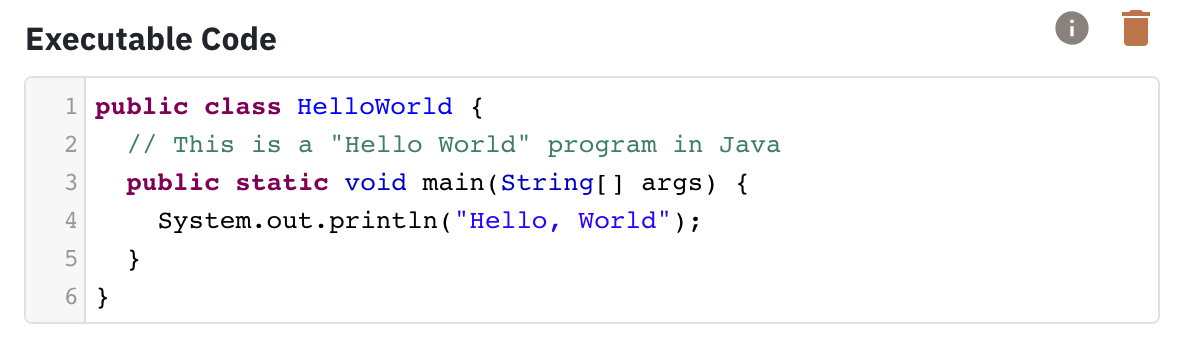
\includegraphics[width=\textwidth-1pt]{chapter/entwurf/bilder/weclare_codemirror.png}}
    \caption[Darstellung eines ausführbaren Java-Quelltexts in Weclare]{Darstellung eines ausführbaren Java-Quelltexts in Weclare mittels der CodeMirror-Bibliothek.}
    \label{abb:weclare_codemirror}
\end{figure}

\newpage
\section{Code-Ausführung im Browser via DoppioJVM}
\label{chap:ausfuehrung}
Normalerweise wird Java in einem zweistufigen Prozess ausgeführt. Zunächst wird eine plattformabhängige JVM geladen. Innerhalb dieser JVM wird der Java-Compiler (javac) aufgerufen. Dieser compiliert Java-Quelltext zu Java-Bytecode. Der Java-Bytecode kann dann von der JVM ausgeführt werden. Dieser Ablauf ist in der \ref{abb:java_execution} unter a) dargestellt.

Um Java in einem Browser auszuführen ergeben sich konzeptionell mindestens drei verschiedene Möglichkeiten, die in \ref{Abbildung 4.4} mit den Buchstaben b-d gekennzeichnet sind.

\begin{figure}[H]
    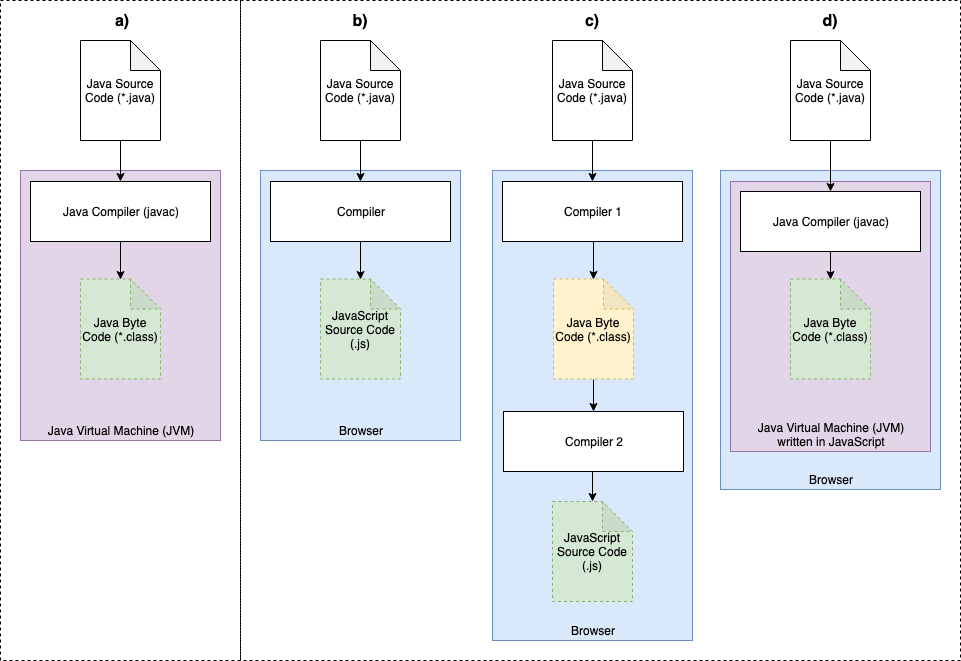
\includegraphics[width=14cm]{chapter/entwurf/bilder/Java_JavaScript_Execution.png}
    \centering
    \caption{Blubb}
    \label{abb:java_execution}
\end{figure}

\begin{itemize}
    \item \textbf{b:} Java-Quelltext wird mit einem Compiler direkt in JavaScript umgewandelt: Diese Variante ist konzeptionell sehr einfach. Zwar gibt es einige Programme, welche Java-Quelltext in JavaScript übersetzen können (zum Beispiel JSweet oder GWT), jedoch sind alle diese Programme entweder in Java selbst oder in anderen Programmiersprachen verfasst. Einen solchen Compiler, der selbst in JavaScript geschrieben wurde, gibt es bisher nicht. Es wäre möglich eines der besagten Programme auf einem separaten Server zu verwenden. Dies würde aber eine weitere Abhängigkeit von einem Server bedeuten, und damit der formulierten Kern-Anforderung widersprechen.
    \item \textbf{c:} Java-Quelltext wird mithilfe eines ersten Compilers in Java-Bytecode übersetzt. Anschließend wird der Java-Bytecode mit einem zweiten Compiler in JavaScript übersetzt. Auch hier ergibt sich das gleiche Problem wie in b). Zwar gibt es Programme, die den jeweiligen Teilschritt übernehmen könnten, jedoch ist keins davon in JavaScript verfasst, so dass es keine Lösung dafür im Browser gibt.
    \item \textbf{d:} Es wird eine JVM verwendet, die in JavaScript implementiert wurde. Mithilfe dieser JVM kann der javac-Compiler geladen werden, um Java-Quelltext in Java-Bytecode zu übersetzen und anschließend auszuführen. Eine solche JavaScript-JVM existiert bereits in Form eines Universitätsprojekt der University of Massachusetts unter dem Namen DoppioJVM. Der konzeptionelle Nachteil dieser Lösung liegt in der benötigten Datenmenge: Um eine komplette JVM im Browser auszuführen wird ebenfalls die Java Runtime Environment benötigt, deren Größe bei etwa 60 Megabyte liegt.
\end{itemize}

In Anbetracht der Tatsache, dass die Ausführung der Code-Beispiele im Browser exakt die gleichen Ergebnisse liefern soll, wie die Ausführung in einer lokalen JVM (zum Beispiel auch in Bezug auf Fehler beim Kompilieren), so ist die Variante d die bevorzugte Lösung und wurde im Rahmen dieser Arbeit in das entstandene CRS integriert.

DoppioJVM ist das Ergebnis der PLASMA-Forschungsgruppe der University of Massachusetts in Amherst, USA. Das Projekt wurde im Jahr 2014 im Rahmen einer wissenschaftlichen Arbeit veröffentlicht und wird von den Autoren selbst wie folgt beschrieben:

\begin{quotation}
„DoppioJVM is a robust prototype Java Virtual Machine (JVM) interpreter
that operates entirely in JavaScript. DoppioJVM implements all
201 bytecode instructions specified in the second edition of the
Java Virtual Machine Specification, supports multithreaded
programs, runs multiple languages that run on top of the JVM, and
implements many of the complex mechanisms and native functionality that JVM programs expect.“
\end{quotation}

Voraussetzung für den Betrieb von DoppioJVM ist ein weiteres Projekt der gleichen Forschungsgruppe: BrowserFS. Dabei handelt es sich um die Implementation eines NodeJS-kompatiblen Dateisystems innerhalb des Browsers. Somit können JavaScript-Programme, die eigentlich für die NodeJS-Laufzeitumgebung gestaltet sind (also Zugriffe auf ein Dateisystem ermöglichen) auch im Browser ausgeführt werden. BrowserFS emuliert ein Dateisystem auf Basis verschiedener Webstandards. So können für den Betrieb der DoppioJVM zum Beispiel die JRE-Komponenten über ein virtuelles Dateisystem bereitgestellt werden, welches auf dem asynchronen Nachladen basiert, oder andere Komponenten der JVM über den LocalStorage des Browsers.

Nachdem das BrowserFS-Dateisystem konfiguriert ist, kann DoppioJVM mit einer relativ einfachen Schnittstelle verwendet werden:

\begin{minipage}{\linewidth}
\begin{lstlisting}
new Doppio.VM.JVM(
  {
    doppioHomePath: "/sys",
    classpath: [".", "/sys/", "/tmp/"]
  },
  (err, jvmObject) => {
    jvmObject.runClass("Loader", [classname], exitCode => {
      if (exitCode !== 0) {
        console.log("JVM exited with an error");
      } else {
        console.log("JVM exited successfully");
      }
    });
  }
);
\end{lstlisting}
\end{minipage}

Die DoppioJVM muss bei jeder Verwendung neu instantiiert werden. Deswegen ist es erforderlich, dass die Kompilierung und Ausführung des gewünschten Java-Codes in einem Aufruf erfolgt. Dazu hat Java einige Möglichkeiten an Bord, die in Form der folgenden Loader-Klasse implementiert wurden:

\begin{minipage}{\linewidth}
\begin{lstlisting}
import javax.tools.*;
import java.lang.reflect.*;
import java.io.*;
import java.net.*;

public class Loader {
  public static void main(String[] args) {
    if (args.length == 0) {
      System.out.println("No class was found.");
      System.exit(1);
    }
    String className = args[0];
    String sourceFile = "/tmp/" + className + ".java";
    String classFile = "/tmp/" + className + ".class";

    System.out.println("Compiling found class '" + className + "'...");

    JavaCompiler compiler = ToolProvider.getSystemJavaCompiler();
    int result = compiler.run(null, null, null, sourceFile, "-d", "/tmp/");

    if (result == 0) {
      try {
        System.out.println("Compilation successful. Executing...");
        System.out.println("---");

        URLClassLoader classLoader = new URLClassLoader(
            new URL[] {new File(classFile).toURI().toURL()}, ClassLoader.getSystemClassLoader());
        Class<?> c = classLoader.loadClass(className);
        Method m = c.getDeclaredMethod("main", String[].class);
        m.invoke(null, new Object[] {});
        classLoader.close();

        System.out.println("Execution successfull");
      } catch (Exception e) {
        e.printStackTrace();
      }
    } else {
      System.out.println("Could not compile");
    }
  }
}
\end{lstlisting}
\end{minipage}

\begin{figure}[H]
    \centering
    \setlength{\fboxsep}{0pt}
    \setlength{\fboxrule}{0.5pt}
    \fbox{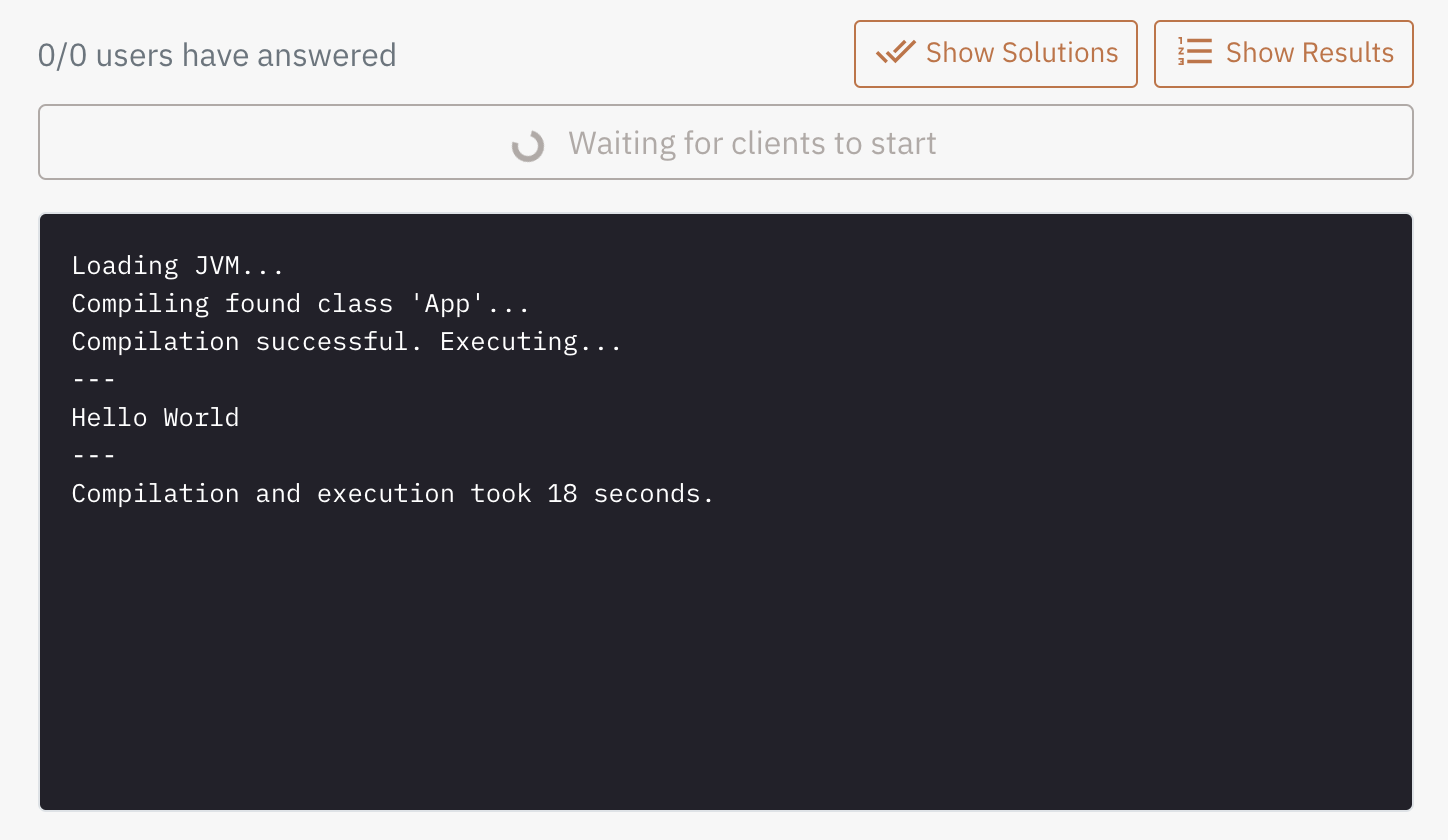
\includegraphics[width=\textwidth-1pt]{chapter/entwurf/bilder/weclare_jvm_console.png}}
    \caption{Ausführung einer Java-Klasse in Weclare mittels DoppioJVM.}
    \label{abb:weclare_jvm_console}
\end{figure}


%
\chapter{Fazit und Ausblick}
\label{chap:fazit}
Für jede der ermittelten Anforderungen soll einzeln erörtert werden, ob die Umsetzung gelungen ist, und welche Erfahrungen bei der Implementierung gemacht werden konnten.

\subsubsection*{Web-Applikation}
Trotz einiger Nachteile, die der Browser als Laufzeitumgebung mit sich bringt, erscheint es sinnvoll und zeitgemäß, ein CRS vollständig webbasiert zu implementieren. Die technischen Anforderungen an das ausführende System sind relativ gering. Die Anforderungen an die User Experience und eine gut gestaltete Benutzeroberfläche im Gegensatz dazu eher hoch. Es erscheint daher nicht mehr zeitgemäß für die technisch relativ simple Aufgabe, die ein CRS bewältigt, Software extra herunterladen und installieren zu müssen (es sei denn es gibt Gründe wie etwa geforderte Hardware-Kompatibilität).

Das React-Framework hat sich als gute Wahl für diese Aufgabe herausgestellt. Die bereitgestellten Konzepte und Bibliotheken waren relativ einfach zu verstehen und haben eine sehr schnelle Entwicklung ermöglicht. Langfristige Wartbarkeit scheint durch die Größe der React-Gemeinde ebenfalls gegeben zu sein.

Eine wichtige Erfahrung dieser Arbeit war der Umgang mit dem enorm großen JavaScript-Ökosystem. Zwar ist die Masse an verfügbaren und kostenlosen, OpenSource-JavaScript-Bibliotheken überwältigend, allerdings zeigt sich, dass es oft schwer ist, stabile und zuverlässige Projekte zu finden. Die Anzahl und Aktivität der Entwickler sowie die Häufigkeit von Updates waren oftmals bessere Kriterien für die Auswahl einer Bibliothek als ihr anfänglicher Funktionsumfang.

\subsubsection*{Peer-To-Peer-Verbindungen}
Die Implementierung von Peer-to-Peer-Verbindungen auf Basis von WebRTC erwies sich als schwierig. Der WebRTC-Standard ist leider noch nicht fertiggestellt, und die Abweichungen zwischen den Implementierungen der verschiedenen Browser-Hersteller sind relativ groß. WebRTC im Produktiveinsatz mit breiter Kompatibilität zu verwenden ist aufwändig, das scheinen auch große Firmen zu sehen: Erst kürzlich aktualisierte Microsoft seinen „Skype for Web“-Dienst mit WebRTC-Technologie. Zunächst wurden dabei alle anderen Browser außer Google Chrome ausgesperrt – vermutlich ist die schwierige WebRTC-Kompatibilität einer der Gründe dafür\footnote{Quelle: \url{https://arstechnica.com/gadgets/2019/03/microsofts-new-skype-for-web-client-an-early-taste-of-the-browser-monoculture/}}.

Die Verwendung von WebRTC-Wrappern wie PeerJS, die die Schnittstelle vereinfachen und das Signalling regeln, erscheint gerade in kleinen Projekten daher unausweichlich zu sein. Leider gibt es bisher nicht sehr viele, und nicht sehr aktuelle Open-Source-Bibliotheken für diese Aufgabe. Es bleibt zu hoffen dass die Stabilität der Schnittstelle und damit auch die Qualität der Wrapper-Bibliotheken nach dem Ende der WebRTC-Standardisierung ein besseres Niveau erreicht.

Das fertige System funktioniert zwar einwandfrei, allerdings kann es schnell zu Komplikationen kommen, zum Beispiel wenn die Verbindung der Teilnehmer während einer Sitzung unterbrochen wird oder wenn Browser-Versionen nicht unterstützt werden.

\subsubsection*{Code-Formatierung}
Die Einbindung von bestehenden, Editor-Bibliotheken war eine sehr gute Entscheidung. Es gibt eine große Anzahl von sehr aktiven JavaScript-Editor-Bibliotheken, allerdings bieten nur wenige davon auch eine überzeugende React-Integration an.

\subsubsection*{Code-Ausführung im Browser}
Weclare zeigt, dass die Ausführung von Java-Quellcode im Browser grundsätzlich möglich ist. Wie praktikabel dieses Experiment im Alltag der Dozenten ist bleibt fraglich. Vor allem das notwendige Laden der Java-Runtime sorgt dafür dass die Ausführungsdauer von Code-Beispielen oft unangenehm lange ist. Bei geladener Runtime können Code-Beispiele meistens innerhalb von 15 bis 30 Sekunden kompiliert und ausgeführt werden. Je nach Geschwindigkeit der Internetverbindung kann sich dieser Wert beim ersten Laden der Runtime auf mehrere Minuten vergrößern.

Probleme:
\begin{itemize}
    \item Unit- und Integrationstest für die Anwendung sind dringend notwendig
    \item Die Instantiierung der DoppioJVM sollte in einem eigenen Thread erfolgen und deswegen in einen WebWorker ausgelagert werden
    \item Freitext-Fragen, wie sie von StuReSy und Doppio unterstützt werden, sind nicht implementiert
    \item Die Visualisierung der erhaltenen Antworten in Form von Diagrammen und der Export als Grafik oder CSV wird nicht unterstützt
\end{itemize}





%%%%%% Chapters End

%% bibliography and other stuff
\backmatter

\typeout{===== Section: literature}
%% read the documentation for customizing the style
\printbibliography
\typeout{===== Section: nomenclature}
%% uncomment if a TOC entry is needed
%% \addcontentsline{toc}{chapter}{Glossar}
\renewcommand{\nomname}{Glossar}
\clearpage
\markboth{\nomname}{\nomname} %% see nomencl doc, page 9, section 4.1
\printnomenclature

%% index
\typeout{===== Section: index}
\printindex

\HAWasurency

\end{document}
